\chapter{Introduction}
\label{chap:intro}


Operating systems simplify the programming of an application to utilize a wide range of hardware.
A main purpose of a modern, UNIX-style OS
is to encapsulate the low-level hardware resources and operations for applications~\cite{ritchie74unix}.
%In modern computer systems, an operating system plays a key role
%of abstracting the hardware for applications. % that are designed to run on a wider range of hardware platforms.
%\fixmedp{be more direct}
%Operating systems \fixmedp{encapsulate?} reduce the complexity of hardware management for an application.
%The abstraction of OSes reduces the burden of average developers
%to program the interface of a physical machine.
%abstract the hardware for applications. %rely on operating systems for abstracting the hardware in OS services.
From the perspective of application developers,
an OS is equivalent to 
%The \fixmedp{from the programmers' perspective} top-down view of an OS is 
an extended machine or a ``virtual machine''~\cite{tanenbaum19os-textbook,dhamdhere2007os-textbook},
on which they can expect a consistent {\em system interface} to program the usage of hardware,
instead of directly interfacing hardware devices.
%which hides the low-level details of the hardware.
 %~\cite[Ch.1]{tanenbaum19os-textbook}.
%In an OS,
%Application developers rely on a set of consistent OS functions, 
%or
%An OS exports a set of 
%{\em system interfaces},
%which encapsulates the control of hardware abstractions,
%as a convenient programming standpoint against hardware abstractions. 
%The OS-level hardware abstractions are controlled by the application developers, 
%using {\em system interfaces} as a convenient programming standpoint~\cite{ritchie74unix}.
%System interfaces free the average programmers from
%%\fixmedp{a little fluffy}
%%getting involved with the
%%\fixmedp{a little informal}
%the low-level details of hardware management~\cite[Ch.1]{tanenbaum19os-textbook}.
%Operating systems presents a comprehensive way for application developers to program the hardware resources.
%allowing the application developers to focus on more important implementation issues in hand.
%For application developers, 
%an {\em operating system} represents an abstract layer, %which abstracts the complex, idiosyncratic hardware,
%which provides a comprehensive way to program against the idiosyncratic hardware.
%Using the hardware abstractions presented by the OS,
%The main abstractions of an OS is to manage and abstract the hardware resources, by defining a set of generic {\em system interfaces} for system programming.
%\fixmedp{move some context into previous sentence}
%Application developers use the defined , to request for the OS-managed hardware resources,
%without knowing the low-level details of the hardware.
%System interfaces simplify programming in user space, and \fixmedp{``allow'' is a weak verb} allow application developers to focus on more \fixmedp{importance is not justified} important development challenges, such as debugging and optimization.
%needs not to learn how to program against the low-level hardware interfaces, as well as to constantly reprogram the applications for new hardware platforms.
%Application developers can simply use the {\em system interfaces} defined by the OS,
%which describe the generic logic of using the hardware:
%which in principle describes the generic logic of 
%to express the requirements and operations on the hardware.
%The system interfaces describe the generic logic of using most of the hardware,
%For hardware components with relatively generic architecture and semantics, 
%such as sharing the CPU cycles, allocating the memory, and accessing various types of IO devices. % such as storage and network cards,
%an operating system can define , which can be used by applications,
%to allocate and access hardware resources.
%either statically or in the run time.
%A commodity operating system, such as Linux or Windows, define hundreds or even thousands of system interfaces~\cite{linux-syscall,freebsd-syscall,win-api}, in order to accommodate the diverse, contemporary hardware.
%For programmability, system interfaces are defined to be as generic as possible, despite the idiosyncracies of hardware resources;
%For example, %in a UNIX-style OS,
%\fixmedp{example of example}
%the \syscall{read} and \syscall{write} system calls
%are designed to 
%to program a regular file, without knowing the physical aspects of file storage (e.g., blocks, tracks, and cylinders),
%or the I/O interfaces determined by manufacturers~\cite{ritchie78unix-retro}.
%OSes facilitate application development and execution.
%in order to fulfill complicated tasks on computer systems.
%Ultimately, \fixmedp{this will be a better topic sentence} OSes simplify the programming of an application
%to utilize a wide range of hardware.
The presence of the OSes has an indisputable benefit on the advance of both applications and hardware devices, for reducing the friction against adopting new inventions.



Specifically, many OSes emphasize on the quality of making applications {\em portable} across different hardware,
simplifying the programming of a distributable application %an one-time effort
on limited hardware options available to the developers.
%Many OSes offer the convenience of developing applications
%that are not tied to specific hardware, or {\em application portability}.
Application portability requires an OS to export a system interface
independent from hardware configurations, such as CPU models, memory sizes, and types of I/O devices.
The only exception is the portability across CPU architectures,
since most OSes restrict applications to be compiled with a choice of ISA (instruction set architecture), such as x86 or powerpc.
Otherwise, application developers would expect an application, built without dependency to specific hardware, to be reusable in an OS regardless of what hardware users choose.
The same assumption on application portability has been shared among many OS standards, including POSIX~\cite{ieee-posix}, Linux~\cite{linux-standard-base}, BSD~\cite{quarterman85bsd}, and Windows~\cite{win-api}. 



%OSes define portable system interfaces
%To be specific, OSes reduce the effort of making an application 
%to facilitate reusing applications on
%different hardware configurations
%(e.g., different CPU frequency, size of DRAM, or number of I/O devices).
%A portable OS hides the distinction of physical hardware,
%except for instruction set architectures (ISAs), which are translated by compilers and ISA-specific macros.
%(i.e., running on different physical machines)
% (i.e., deduplicating programming efforts).
%\fixmedp{need a last sentence to connect to the next paragraph}
%Similarly, the POSIX file operations, including \syscall{read} and \syscall{write},
%are used to \fixmedp{``perform'' is a weak verb} perform generic IO operations,
%namely to read in and write out the data, in the ways corresponding to the types of IO devices, such as storing on a disk, or transmission over a NIC (network interface controller).
%Another example is the POSIX-style file system operations, including  \syscall{open}, ;
%these system calls can be generically used for the common IO operations,
%over various types of devices, such as .
%Using these abstractions of hardware, application developers can simplify the development process, as well to reuse the implementations across hardware platforms.
%Besides for the programmability,
%Programming with
%\fixmedp{heavy on ``the''}
%the system interfaces facilitates the reuse of applications
%across different physical machines.
%The top-down view of a modern OS can be portrayed as an extended machine or a ``virtual machine''~\cite[Ch.4]{dhamdhere2007os-textbook},
%which hides the low-level distinction of the hardware.
%The benefit of this design is that an application developer only sees an extended machine with consistent OS functions when programming.
%instead of the distinction of hardware.
%For portability,
%The UNIX standard brings an advantage by
%An early design point of UNIX is to 
%moving a large amount of device drivers
%into the OS space, and defining a set of unified interfaces to encapsulate the device operations~\cite{ritchie74unix}.
%Portability also assists the distribution of software;
%an early design point of UNIX is to help making a program small enough to fit into
%removable disks and be distributable.
%\fixmedp{this  is a different point}
%I/O devices, anonymous pipes, and network sockets are treated indifferently in
%an ``everything-is-a-file-descriptor'' fashion.
%the differences between ordinary files and I/O devices.
%for example, in UNIX-style operating systems, application developers use \syscall{clone} and \syscall{mmap},
%to allocate tasks and virtual memory areas (VMAs),
%to request for CPU and memory resources from the OS.
%The application binaries also contain statically-defined code and data segments, which represent the minimal memory usage to start an execution.
%or based on the code and data segments inside of the application binaries.
%can help splitting the CPU cycles or the physical memory, by allocating task contexts or virtual memory regions inside of an application.
%An application developer can use \syscall{read} and \syscall{write}
%works invariably on 
%\fixmedp{not exactly correct}
%on every readable-writable file descriptors,
%whereas
%the triggered operations can vary from accessing storage blocks to processing I/O %streams.
%POSIX later
%\fixmedp{a little informal; a more formal word: to reinforce}
%reinforces the portability of UNIX by defining a system interface standard that covers ``all'' %the typical hardware operations.
%Similar initiatives are taken by other open OS standards, such as BSD and Linux~\cite{quarterman85bsd,linux-standard-base}, and even close-sourced OSes, such as Windows.
%and some close-source OSes, \fixme{find citation} such as Windows.
%and even close-source OSes, such as Windows.
%In the current OS ecosystem,
%In most of the modern OSes, a developer can easily write a
%\fixmedp{the helloworld example is underselling}
%C program that prints ``hello world'' on any physical machines, in merely five lines of code.
%By making an application portable, the developers eliminate the cost of customizing the application for each physical machines.
%The portable OS design has led the application development for decades.
%A portable OS decouples application development with choice of hardware.



Unfortunately, in a modern OS, system interfaces are not only design to keep future applications portable, but also preserved for the {\em compatibility} against previous applications.
Due to the rapid growth of applications and hardware devices,
OS development is increasingly burdened with implementing the ``legacy'' features and abstractions of the past generations, and can not easily change or deprecate any system interface which may impact applications.
%One reason has been that an OS now has to always keep the system interface {\em compatible} against existing applications,
%instead of just focusing on making new applications portable.
%The amount of applications previously developed in an OS, such as Linux or Windows,
%has grown to untraceable level.
Any change of the system interface will take a long time before updating all the previous applications, potentially causing the adoption of a newly ported OS version to lag behind the development. %for adopting new hardware.
%In a portable OS, application developers no longer have to program
%against each physical machines,
%but instead rely on a set of well-defined, consistent
%system interfaces.
%for clear, consistent OS functions. 
%In a portable OS, application developers only has to be concerned about
%the consistency of OS functions within
%system interfaces. %, instead of portability against hardware.
%with clear, consistent functions.
%It is the responsibility of the OS to ensure a singular programming interface to an application,
%which will not change whenever or wherever
%the application is executed---a quality generally known as
%{\em compatibility}.
%to ensure  to all OS services.
%Compatibility can be simply defined as whether or not an OS contains the necessary system interfaces for specific applications.
%Compatibility requires
%OS developers to preserve all the existing system interfaces, which are currently used by certain applications in operation.
%For decades,
%the ``portable'' design has dominated OS development, %design taken by many OSes %has dominated OS development,
%and obliges new OS extensions
%to preserve the {\em compatibility} of system interfaces. % for applications.
%For an open OS such as Linux or BSD, maintaining the compatibility simplifies
%the OS development post-release,
%which is mostly incremental and distributed.
%lots of applications are developed within the portable system interface standards, and become ``legacies'' of the OSes.
%OS developers have to preserve the {\em compatibility} of system interfaces, to keep all the existing application artifacts reusable
%System interfaces is a ``legacy'' to an OS, and has to be preserved for the reuse of existing application artifacts
%and impacts the reproducibility of existing application artifacts,
%--- a quality also known as {\em compatibility}.
%Individual OS developers who make progress on extending or porting an OS for new hardware are not eligible for
%redefining the existing system interfaces.
%Coordination with a large community of application developers on changing a system interface is usually time-consuming
%so any change of system interfaces is likely to be
%a time-consuming decision 
%made by the whole community of contributors~\fixme{more citations}
%~\cite{corbet15syscall2038}.
%and can affect the usability of existing application artifacts.
%in the OS. %become obsolete afterward.
%A commercial OS such as Linux contains thousands to millions of
%{\em native} applications~\cite{ubuntu-packages},
%which are tied to specific system interfaces. 
%A typical commodity OS, such as Linux, Windows, or OS X, has produced
%thousands to millions of  applications for its users~\cite{ubuntu-packages,ms-by-number}.
%Preserving the {\em compatibility} for applications prevents the applications from becoming obsolete on newer generations of the OS.
%As the OS developers may continue to extend the OS implementation,
%System interface compatibility has been
%application developers need to rely on compatibility as 
%a ``contract'' between the two communities.
%OS developers, to ensure that the future versions of the OS will faithfully implement the same system interfaces used in an application.
The key problem is, application developers need to trust an OS to reproduce consistent functionality for an application,
as it is programmed and tested on the developers' machines.
%on a specific version of the OS.
%will behave consistently on the successors of the OS.
Fulfilling the compatibility of system interfaces
becomes an obligation of OS developers, to ensure the stability of application deployment.

For OS and hardware developers, the requirement of application compatibility is often a distraction to innovations.
%For OS developers, maintaining compatibility is a valuable effort, 
%but also can be a distraction to innovations.
%Normally it is simpler %not particularly difficult
%to extend an OS
%within the realm for which system interfaces are originally designed.
%Although existing system interfaces can cover most
%of the typical hardware operations, it can't avoid leaking new hardware with unprecedented operations or constraints.
%There is a trend that retaining compatibility has gradually become a pain in the OS development, due to the increasing variety among physical machines as well as among applications.
%The focus on convenience of application programming and portability in the OS design space ends up creating several millions-line-of-code OS artifacts,
%including Linux and Windows.
%iThe design of portable system interfaces can't avoid leaking new hardware or OS designs with unprecedented constraints. % or methods of operation.
The early UNIX systems are reportedly easy to implement and evolve, because
%they only have a relatively small amount of hardware devices and applications to deal with, and 
the system interface is tailored
for applications and hardware devices available at the time~\cite{ritchie78unix-retro}.
%The problems lies in the complexity of 
Application compatibility becomes an issue
when new hardware designs leak out of the typical abstractions
encapsulated by an OS.
When changing the system interface becomes unavoidable,
%OS developers have to either extend the existing system interfaces
%to support new hardware,
%or implement a transparent layer which compensate for the distinction.
it would almost certainly delay the timing when users can benefit from the new hardware designs.
A classic example is the Intel SGX (software guard extensions) technology~\cite{intelsgx},
which allows applications to protect themselves from untrusted OSes and administrators,
but requires changing the applications to defend against malicious OS services.
From the experience of porting applications to SGX,
we can observe the challenges for preserving compatibility on an innovative hardware design,
besides simply adapting for ISA distinction.
A key challenge is to adjust the OS architectures or assumptions,
such as making the OS untrusted.
The size and subtlety of system interface in an OS is also unfriendly for OS developers to make a system-wide OS change transparent to applications.
More details about the compatibility issues of SGX are discussed in \S\ref{sec:intro:sgx}.




\begin{comment}
% technologies, because of inevitable modifications to existing applications.
%The latter approach, however, can be challenging for OS developers
%and even be ineffective or inefficient.
Take the Linux support of huge pages (pages larger than 4KB) for example.
%As huge pages are not necessarily beneficial to all memory mappings,
Linux implements a transparent mechanism to convert contiguous 4KB pages to huge pages, in order to keep \syscall{mmap} compatible with existing applications.
The transparent conversion increases paging latency 
and has fragmentation and fairness issues~\cite{kwon16ingens}.
Linux also introduces a new flag \code{MAP\_HUGETLB} for \syscall{mmap}, as an incompatible but more effective way to allocating huge pages.
%, which is more effective and efficient.
Overall, OS developers face a dilemma between preserving the compatibility for existing applications and extending system interfaces for abstracting new hardware.
The development effort of preserving the compatibility may be too expensive,
or violate the performance or threat models of certain native applications, making the transparent approach no longer an option.
Because updating all application against the new system interfaces
can be time-consuming,
%Although redefining system interfaces can %fundamentally
%solve the issues of porting,
%updating affected applications is time-consuming, and 
OS developers should not delay and let the perfect be the the enemy of the good.
%when deploying new hardware. 
\end{comment}

%An example of the fall-back support is the implementation in Linux to support huge pages , which transparently converts contiguous 4KB pages to huge pages, for VMAs allocated with the old \syscall{mmap} (without using the newly-added \code{MAP\_HUGETLB} option).
%Linux also adds a new system interface---a  to \syscall{mmap}---which is much more efficient,
%because the OS needs not to guess which VMAs can benefit from huge pages,
%but does not supersede the fall-back strategy.

\begin{comment}
Nowadays, any commercial-class OS has to contain at least thousands of device drivers~\cite{padioleau2008linux-device-drivers}, to accommodate the diversity of hardware options among physical machines.
The system interfaces have also grown way more larger than the original UNIX interfaces, and offered much more programmable options (i.e., flags and opcodes),
in order to adopt new hardware or
to optimize for corner cases in applications~\cite{linux-man-syscall,win-api,ieee-posix}.
OS developers are in fear of disrupting the support for existing applications, and thus have to avoid changing any part of the system interfaces.
For a well-adopted architecture such as x86, the Linux developers cannot change or retire a system call before spending at least six years to confirm that no application uses the system call.
Otherwise, the extensions to the OS must be always transparent to the existing system interfaces.
The implementation of an OS is then complicated
by supporting the system interfaces that are not defined with the new hardware in mind.
%even though the system interfaces are not necessarily defined with the new hardware or new OS design in mind.
As two examples of the commodity OSes, both Linux and Windows have grown to overwhelming complexity,
in the order of millions of lines of code
%the modern OSes, including Linux and Windows, are as complex as a %piece of several-millions-line-of-code software
~\cite{tanenbaum2006os,kroah2007linux,cusumano1997microsoft}.
\end{comment}

%However, the increasing variety of applications and physical machines
%has raised the bar for retaining OS portability.
%A commercial-class OS has to contain at least thousands of device drivers~\cite{padioleau2008linux-device-drivers}, each of which will transparently implement a set of legacy driver interfaces.
%Each device driver is a transparent implementation of the legacy driver interfaces, in order to be pluggable to the OS.
%In addition, system interfaces have grown much more complex and offered more programmable options, as being tailored to the need of applications.
%The modern versions of Linux, Windows, and POSIX have each defined hundreds to thousands of OS functions~\cite{linux-man-syscall,win-api,ieee-posix}, to support a tremendous amount of existing applications. 


%Linux contains more than three hundred system calls;
%in Windows 8.1, the core system libraries (e.g., \code{nt.dll}) export more than four thousand APIs;
%, which includes the APIs exported by the core system libraries, contains more than four thousands interfaces;
%even POSIX has raised the number of APIs to 1,191, in version 1003.1










\begin{comment}
A hardware platform consists of various types of hardware, including CPUs, memory, and I/O devices. Users select the hardware platforms %to run the OS and application,
based on their specification and budget.
Reusing an application
%An application that targets multiple hardware platforms
%of the hardware products, at a reasonable budget.
%The OS essentially decouples this choice of hardware platforms from the applications.
can loosen the restriction on selecting hardware platforms,
and thus multiplies the value of the application.
%by reusing the same application code written by the developers.
%Hardware platforms can contain hardware components
%of different capacity and performance.
%A generic system interface can conceal the difference of hardware platforms,
%, and makes applications reusable as long as they are programmed against the same system interfaces.
%and allow application developers to decouple the development process
%from the choice of hardware;
To put into context, an application developer can expect her application to work on either a single-core Pentium-4 3.4GHz CPU or an 8-core Xeon E5 1.8GHz CPU, with no difference, except for the impact on performance.
Using \syscall{clone} and scheduling APIs (e.g., \syscall{sched\_setparam}), the difference of the CPUs is orthogonal to the reusability of applications.
%application can be reused above difference number of CPU cores, or different CPU frequency, 
%and the choice of CPU will look no difference to the application,
%can look no difference to an application that simply uses \syscall{clone} to create new threads for parallel processing, 
%as long as they have the same instruction set (e.g., x86).
%More importantly, the application developers should not have to reprogram the application against each CPU, except for another instruction set architecture (such as x86 to ARM). 
%Reimplementing an application for every choice of hardware made by the users is a expensive cost that application developers cannot possibly afford.
%Sometimes, a language runtime, such as a Java virtual machine (JVM), may impose another layer to reuse applications across OSes and instruction sets, but still relies on system interfaces of each OS, to make the whole language runtime reusable across hardware platforms.
%abstract the hardware resources, as well as to keep the language runtime itself reusable across hardware platforms.
%as well as to keep the runtime itself platform-independent.
%By wrapping the hardware operations with generic system interfaces, 
Using system interfaces, application developers can avoid writing the platform-specific code for hardware management, in either an application or a general-purpose, linkable library.
%Developers may even write a general-purpose library, such as a cryptographic library, to be reusable in arbitrary applications,
%and thus can make the library code more broadly reused on hardware platforms.
\end{comment}

%Only a few hardware components require specialized system interfaces or tool-chains to program against;
%for example, recently Intel CPU extensions, including SGX~\cite{intelsgx} and MPX~\cite{intelmpx}, require applications to access a set of customized opcodes to the Linux's \syscall{ioctl} system call,
%or be explicitly compiled against specific compiler options (e.g., ``\code{-mmpx}''~\cite{intelgccmpx}).
%Another example is a GPU (Graphic Processing Unit),
%which requires applications to be partially reprogrammed in a different language, such as CUDA~\cite{cuda}. 

\begin{comment}
The modern OSes face a challenge as retaining the {\em compatibility} to the existing applications,
in order to preserve the legacy of software development.
%This thesis defines 
%\fixme{define ``compatibility''}
%the quality of reusing formerly-developed applications on different hardware platforms, as {\em compatibility}.
%To keep the system interfaces programmable, the OS is obliged to maintain the consistency of system interface, or , to ensure continuous support to applications.
%The programmability of system interfaces has a caveat: applications require the OS developers to be disciplinary on avoiding the disruption on the system interfaces used by the applications, or, in other words, keeping the OS {\em compatible}.
%In order to preserve the {\em reusability} of applications, the application developers require the OS the 
%Compatibility is critical to all production OSes %because it directly affects whether the customers can continue to run the same applications.
%because application developers cannot afford re-implementing the applications
%whenever a new OS version is released. %implementation is updated, in order to support a new hardware platform.
Compatibility relies on %both genericity of system interfaces and {\em backward compatibility} of the implementation.
%For genericness, the application needs the system interfaces to be independent to the hardware platforms.
%For backward compatibility, the application expects 
the OS to faithfully implement the existing system interfaces,
to prevent the OS updates from making the existing applications obsolete.
%The consistency of system interface implementation is also called ``{\em backward compatibility}'', to differentiate with compatibility.
Compatibility is essentially a long-lasting ``contract'' between the OS and the application developers.
%Application developers expect the system interfaces to stay identical;
A compatible OS ensures that
all previously developed and tested application will behave consistently on the successors of the OS.
%identically on the same OS installed on other hardware platforms.
%Unless the OS has finished its development cycles and stop to adopt new hardware platforms, the compatibility has to be always maintained by the OS developers.

%can have the same behavior, on the OS versions for programming and testing, as well as the ones installed by the users.
%If the OS fails to maintain the compatibility, the users mostly do not have the expertise of updating the application implementation, or the budget of paying the developers to do so.
%The user can end up sticking to the older version of the OS, or even switching to another OS which has superior compatibility and can support the application on the desired platform.
%Users of an application are also likely to stick to an OS that is compatible to the application, than switching to a newer, but incompatible OS.
%To avoid reprogramming applications for every new hardware platform,
%an operating system is responsible for maintaining the {\em compatibility} of its system interfaces, regardless of what the underlying hardware is.
\end{comment}



%These two principles, backward-compatibility and portability, both contribute to the reuse of applications,
%but can occasionally become contradictory.


%not only program but also test the applications against the certain system interfaces.
%The other factor of OS compatibility is to keep the system interfaces generic to the hardware, even beyond the introduction of new hardware.
%The constant factor is to reduce either the risk or the effort that application developers have to reprogram a released application, at any timing during the OS development cycle.
%We differentiate OS compatibility from hardware compatibility as well as
%other levels of compatibility in individual applications.

%On the other hand, the system interfaces that the operating system formerly defines have to accommodate future hardware as much as possible (i.e., {\em forward compatibility}). 
%If OS developers fail to maintain either the backward or forward compatibility
%in an evolving operating system, application developers may be forced to reprogram their applications at a certain point of time,
%to match with the new system interfaces designed to accommodate the outliers.
%The penalty of failing the compatibility can be huge: Among the worst consequences, an operating system can lose its users,
%if the users can no longer run the desired applications, unless they pay the cost of reprogramming.


%\fixme{switch to the OS perspective}
%From the perspective of OS developers, fulfilling the two meanings of OS compatibility, keeping the OS {\em generic} and keeping the OS {\em backward-compatible}, can be contradicting. 


%In fear of breaking the compatibility,
%OS developers are reluctant to introduce any disruptive OS designs or research concepts
%which may change the system interfaces.
%For an OS, implementing compatibility is both high-stakes and high-priority.
%failing the compatibility may cause the OS to lose users who want to run an application that cannot be reused.
%Compatibility is the first factor that decides whether an OS is usable to a user, as the user cares about whether she can run the desired applications.
%on the target hardware platform. %Therefore, OS developers often go to great lengths to preserve the compatibility of a OS.
%In Linux or Windows, great effort has been made to avoid changing the behavior of an existing system interface, as well as to avoid deprecating one.
%in order to preserve the backward compatibility.
%Instead, they add new system interfaces, or extend the old system interfaces with new corner cases, without disrupting the implementation of existing system interface behavior.
%The limitation is especially problematic, when the old system interface can no longer accommodate the operations on the new hardware.
%In this case, the OS developers are forced to add new system interfaces, or add new corner cases to the old system interfaces, without touching the old system interfaces.
%OS developers must abide with the compatibility of the existing system interfaces,
%and only add or extend system interfaces for supporting new hardware.
%, so that the old system interfaces can remain unchanged.


\begin{comment}
%If an OS must introduce new system interfaces to support new hardware, old system interfaces are kept around for compatibility, creating system interfaces with duplicated functionality.
%OS developers often choose to add new system interfaces, while keeping the old ones around as duplicates.
%The duplication of system interfaces complicates the OS development, because the OS has to implement the new system interfaces for extended hardware support,
The compatibility requirment also restricts an OS developer to add system interfaces for supporting new hardware platforms.
Because only an updated application can benefit from new system interfaces, an OS developer has to to implement a transparent, ``fall-back'' support, for an existing, unmodified application %using the outdated system interfaces, 
to utilize the new hardware.
%in order to support a new hardware.
%In order to preserve an old system interface with the support of new hardware, OS developers often implement , which will compensate for the existing applications.
%existing applications that use the old interfaces and the new applications that use the extended interfaces.
%Sometimes, the OS developers have to implement a ``fall-back'' mode, to ensure that the existing applications can still use the old system interfaces, 
%even though these system interfaces are supported 
%under the emulation of the OS.
%Implementing the fall-back mode for new hardware can be challenging;
An example of the fall-back support is the implementation in Linux to support huge pages (pages larger than 4KB), which transparently converts contiguous 4KB pages to huge pages, for VMAs allocated with the old \syscall{mmap} (without using the newly-added \code{MAP\_HUGETLB} option).
%Linux also adds a new system interface---a  to \syscall{mmap}---which is much more efficient,
%because the OS needs not to guess which VMAs can benefit from huge pages,
%but does not supersede the fall-back strategy.
The fall-back support is usually less efficient and complicates the OS design, 
just like the conversion for huge pages would bring overheads to the page fault handler.
However, OS developers cannot let the perfect be the the enemy of the good.
A slightly slower but compatible solution, in many cases, is a necessary evil, in order to maintain the reusability of existing applications.
\end{comment}

%Using the \code{MAP\_HUGETLB} option is more effective than transparent conversion, because the OS needs not to anticipate whether the VMAs will benefit from using huge pages.


\begin{comment}
In case an OS has to change or deprecate a system interface, the OS developers might emulate the system interface in a user-space library.
In Linux, the GNU standard C library (i.e., \code{glibc}) is often responsible for maintaining the compatibility of the system call table;
\code{glibc} contains several wrappers for retired system calls, such as \syscall{fork} as a wrapper to the more general \syscall{clone} system call.
%using wrappers to the existing system calls (e.g., \syscall{clone}).
%For example, \syscall{fork} is replaced by a wrapper in \code{glibc}, to explicitly call \syscall{clone} without the \code{CLONE\_VM} option (equivalent to \syscall{fork}), so that the old applications using \syscall{fork} can still be supported.
If library emulation is difficult, the OS might even introduce a compile-time tool, to rewrite or to recompile the application code
against the new system interfaces. %The tool chain will technically make the application code reusable, but can no longer reuse the previously-compiled binaries.
Virtualization is also a slightly more expensive solution to maintaining compatibility;
for example, Windows 7 supports a compatibility mode for reusing the XP-only applications, or ``XP mode'', which internally runs the applications in a virtual machine.
\end{comment}

%Unfortunately, the recent trend of hardware technology shows
%that it is getting increasingly difficult to keep the system interfaces compatible, while adopting all he new hardware.

%follow both principles: to make the system interfaces both backward-compatible and generic.
%Unfortunately, the feasibility of maintaining compatibility in a commodity operating system is reaching a tipping point, as the latest hardware does not necessarily follows the same semantics.
%A set of formerly-defined system interfaces does not always accommodate
%the operations of new hardware.
%\fixme{back this claim}


%For example, the latest CPU technology is that
%computer architects are more aggressively introducing new instruction set extensions into commodity CPUs, to compensate for the slowdown of Moore's Law, and to utilize the spare transistors on new generations of CPU chips~\cite{baumann17hotos}.
%Recent Intel CPU extensions, including SGX~\cite{intelsgx} and MPX~\cite{intelmpx}, require applications to use a set of new opcodes to the Linux's \syscall{ioctl} system call,
%or be explicitly compiled against specific compiler options (e.g., ``\code{-mmpx}''~\cite{intelgccmpx}).
%\fixme{this sentence requires citations to back the claim.}
%Studies also confirm the increasing likelihood of using heterogeneous hardware
%in future systems, as many latest cloud providers or embedded systems have begun to install their machines with accelerators, general-purpose GPUs, programmable hardware (e.g., FPGA), or peripheral devices (e.g., DRAM, storage, or NICs) with near-data processing.
%An \fixme{use a different adjective} eccentric processing unit, such as GPU, will require developers to wholly or  partially reprogram the applications in a different language, such as CUDA~\cite{cuda}.
%The evolution of hardware poses a huge challenge to maintaining the compatibility in operating systems, since the existing system interfaces are simply not enough to accommodate all the new hardware.
%Driven by this hardware trend, OS developers of Linux and Windows have both rapidly expanded their system interfaces, by both the number of interfaces and the complexity of control options,
%while keeping the old interfaces around for backward compatibility.
%Both Linux and Windows have recently experienced explosive growth on the number of system interfaces, which reflects this trend.

\begin{comment}
%Besides maintaining compatibility of the existing system interfaces in an OS, it is common that a new, research OS prototype to implement the compatibility to a production OS (we call the quality {\em inter-OS compatibility}).
Compatibility also matters for reusing applications developed for a production OS, such as Linux or Windows,
on a new OS prototype or another production OS.
The purpose of ``inter-OS compatibility'' is  to adopt the collection of applications that are only available on another OS.
For an OS prototype, the developers have the opportunity
to redefining all system interfaces, which allows introduction of innovative concepts or programming models.
Even between production OSes, such as Linux, Windows, and OS X, inter-OS compatibility are developed as features, such as the Bash-On-Windows to run Ubuntu applications in Windows, and the WINE emulator to run Windows applications in Linux or OS X.
%Maintaining compatibility is also a challenge for the development of a new OS prototype, often for research purposes.
%OS researchers feel the need of building new operating systems
%because existing operating systems, such as Linux or Windows,
%pile up too many idiosyncratic, over-complicated behaviors and implementations, after being used and developed for decades.
%Many innovative OS concepts, data structures, and programming languages cannot be introduced to these operating systems
%without rewriting a significant potion of the kernel code.
%\fixme{cite exokernel, microkernel, IX, and Arrakis}
%Previous research work has point out that the existing commodity operating systems are too complex, so that it is hard to verify or reason about the performance or security of an operating system, or too expensive to process IO requests across the whole system stacks.
%\fixme{cite the Rust kernel paper and HotOS paper}
%Also, a new programming language, such Rust, can potentially be a better choice than the C language for OS development, due to the security features,
%but it is too hard to reprogram the whole operating system in a completely different language.
%So far, OS researchers have succeeded academically on building OS prototypes
%to demonstrate more superior OS designs and implementation.
%However, in order to make these OS prototypes applicable to all existing applications, a long and painful process of development is almost unavoidable. 
\end{comment}


\begin{comment}
However, implementing compatibility can cause a dilemma, when supporting a new hardware platform that affects a large amount of system interfaces.
For example, an unconventional memory architecture, such as NUMA (Non-uniform Memory Architecture) would affect every system interface that access shared, kernel state across memory units.
%OS developers face a dilemma when implementing compatibility of the OS:
%due to programmability, application developers require the system interfaces to stay generic and backward-compatible; however, OS developers also need to continue the OS development, in order to support new hardware platforms.
%The primary challenge to implementing compatibility,
%with a new hardware platform,
%is the complexity of updating the current OS implementation to the system interfaces, which are unchangable and often overly complex.
%in a commidity OS such as Linux or Windows.
%is to provide the complete support of the enormous and complex system interfaces of a production OS.
As another example,
the Intel SGX (Software Guard Extensions) moves an application into an isolated environment protected by the CPU, and treats all system interfaces
provided by the OS as untrustworthy.
Supporting these new hardware platforms, for the existing, unmodified applications, 
poses a tremendous challenge for OS developers.
OS developers have to update a substantial portion of the OS implementation,
without disrupting the support for existing system interfaces.
The OS development process can be both painful and time-comsuming.
\end{comment}



Application compatibility also raises challenges for the development of a new OS prototype,
especially for experimenting an innovative OS design~\cite{baumann09barrelfish,unikernels,zeldovich+histar,libra,peter14arrakis,belay14ix}.
For practical reasons, 
an OS prototype often chooses to implement system interfaces of a popular OS standard, such as POSIX or Linux, to reuse applications already under deployment.
%It is a practical move to implement system interfaces from a popular open OS such a Linux,
%to demonstrate the benefits of using an OS prototype
%on running certain native applications.
An OS standard can contain up to hundreds or thousands of functions in the system interface~\cite{ieee-posix, linux-man-syscall},
which is nearly impossible to fully implement from scratch.
Sometimes, virtualization can help reusing a whole Linux kernel on a OS prototype~\cite{baumann09barrelfish}, but depends on hardware support like VT, and costs lots of memory to run an unmodified kernel~\cite{agarwal15container}.
For an OS prototype which prefers not to run a whole Linux kernel, making it compatible against existing applications is a major challenge to moving the OS toward production.


\begin{comment}
The problem to building an OS prototype with compatibility is in the complexity
of system interfaces that have to be implemented.
%A primary challenge to implementing compatibility on these disruptive hardware platforms
Linux, for example,
%A commodity OS, such as Linux or Windows, normally contains a large amount of system interfaces. %, with significant complexity.
%The Linux kernel defines 
contains about three hundred system calls,
each of which 
can further define several options, sub-interfaces (e.g., opcodes for \syscall{ioctl}), and corner cases.
%, which includes the APIs exported by the core system libraries, contains more than four thousands interfaces;
%Even for a POSIX-compliant OS, such as AIX, 
POSIX also contains up to 1,191 APIs (version 1003.1)~\cite{ieee-posix}, if the OS prototype is meant to be POSIX-compliant. % including the extensible \syscall{ioctl}.
%many of these interfaces have defined a tremendous amount of features, control options, sub-interfaces (e.g., opcodes for the \syscall{ioctl} system call), and corner cases.
%Reimplementing the whole system interfaces in another production OS, or a research OS prototype, is a huge burden to the OS developers.
%Many decisions made in the definitions of these system interfaces are random and inconsistent,
%making the implementation of the interfaces in a new operating system an unbearable pain.
Similarly, in Windows 8.1, the core system libraries (e.g., \code{nt.dll}) export more than four thousand functions~\cite{win-api}.
These OSes or OS standards have defined objectively large system interfaces, which would be
%difficult to preserve when updating a substantial part of the OS implementation.
expensive to implement on
 a new OS prototype.
\end{comment}



%The second reason is more nuanced but has a deep impact on
%OS prototyping: the development of commodity operating systems has always been driven by certain conventional models and assumptions, which can be too limited or too outdated.
%For instance, a commodity operating system always assumes a ``monolithic'' kernel, which is privilege-separated by the hardware from the address spaces of applications.
%The monolithic kernel must be trusted by all applications that run on top of it, and is assumed to be secure and correct, for implementing all system interfaces that the applications depend on. Some modern computer systems oppose this model;
%\fixme{citations needed}
%Running a monolithic kernel can be too expensive for hardware platforms that have a limited resource or energy budget;
%Otherwise, an application can be too sensitive to run on a kernel
%that is too complex to defend any exploitable vulnerabilities.
%Another assumption always made by a commodity operating system is the presence of
%the traditional Von Neumann architecture, where the CPUs always run on top of a coherent memory architecture.
%Some research OS prototypes, especially ones that are designed for hardware heterogeneity or parallelism, insist on not assuming a shared, coherent memory,
%to avoid expensive inter-processing-unit communication.



% Operating systems (OSes) have been essential to running applications on most hardware since the 1960s~\cite{hansen10osbook}. Before OSes are invented, applications are programmed to run directly on hardware, while developers simply exchange reusable code (i.e., \emph{libraries}) for hardware drivers or common operations~\cite{silberschatz08osbook}.
% As computer systems become more and more complex, applications begin to require a piece of OS to securely share hardware resources between each others, and obtain a bank of useful APIs (application program interfaces) at developers' disposal.
% Modern OSes like Linux, Windows and Mac OS are ubiquitous and indispensable to \emph{millions} of applications, respectively~\fixme{cite statistics}, by providing a wealth of OS features such as scheduling, memory management, storage and networking.


%In addition, maintaining compatibility against existing applications is also a challenge for OS prototypes built for exploring new OS architectures.



%The applications of a commodity operating system, such as Linux or Windows,
%represent the research space for practical, what-you-build-is-what-you-use system development.
%Recent system researchers increasingly use Linux as the backbone of prototyping, for shortening the time elapsed before integration into production systems.
%Compared with other operating systems, Linux is particularly popular among system researchers due to practical reasons, besides being free and open.
%Firstly, Linux supports a sufficient sized software collection ready for commercial-purpose deployment. More importantly, Linux has been broadly ported to almost every domains of computation environment, including from mainframe and desktop computers, to mobile and embedded devices\fixme{cite some study}.
%Overall, Linux provides a stable research environment, which is versatile enough for experimenting new hardware or OS designs, as well as mature enough for showing the practicality.


% The versatility of Linux comes with an important caveat---Every system researchers devoted to using Linux for prototyping are responsible for preserving the compatibility of the Linux interfaces.
% The development of a new Linux kernel, either partially or completely modified, cannot affect the reusability of existing applications running on top of previous Linux kernels.
% The common practice is, 

 
%\fixmedp{Make one point at a time}
%Operating systems manage and abstract hardware resources (such as CPU time, memory, and IO devices) and OS resources (such as credentials and FIFOs) for applications. \fixmedp{start from the application perspective} Applications access hardware and OS resources through generically-defined system APIs (application programming interfaces). Using the system APIs, applications can allocate and access hardware resources, without assuming the capacity or design of the hardware. For example, by calling the threading APIs (e.g.,  \funcname{clone}), applications can obtain fair share of the CPU time and concurrency, without knowing the number of CPU cores. Applications also uses device-neutral system APIs, such as the \funcname{read} and \funcname{write} system calls, to unanimously access a variety of IO devices, such as storage and network devices. In general, application developers rely on the portability of the OS, to design applications that can be reusable across hardware platforms.




%The hardware resources on hardware platforms often differ from one another. The OS, in general, is responsible of mitigating the inconsistency, to allow applications to be reused across hardware platforms.  For instance, the OS schedules and virtualizes CPU and memory resources to applications, using threading and memory paging. The OS also hides the idiosyncrasy of hardware interfaces behind the system interfaces. Applications use generically-defined system interfaces, such as the \funcname{read} and \funcname{write} system calls, to unanimously access IO devices. In current operating systems, developers build general-purpose applications without assuming the hardware setup.


%\fixmedp{OS perspective: how to maintain portability}
%The OS achieves cross-platform portability by hiding the idiosyncrasy of hardware resources behind system APIs. For some hardware idiosyncrasy, such as the ISA (instruction set architecture) of each CPUs, are mitigated by compilation, either statically or just-in-time (JIT), and deploying architecture-dependent binaries. For other hardware, the OS generally virtualizes the hardware resources by defining the general structures and behaviors of the hardware: CPU and memory resources are managed in threads and virtual pages, respectively; The space on stroage devices in distributed into files and directories; The bandwidth on network devices are shared among network sockets created by applications. To translate the hardware semantics to the virtualized resources, the OS internal is filled with drivers, as well as the general logic for scheduling the resources among applications. For instance, Linux kernels use the {\tt block\_device\_operations} structure to implement the translation for each storage devices. The {\tt block\_device\_operations} structure is then used by VFS (virtual file system) operations to support system calls like \funcname{read} and \funcname{write}. To maintain portability, the same type of hardware devices must behave in similar ways, with little flexibility of customizing the hardware interfaces.  


%The OS schedules the applications to run on each CPU cores. The virtual memory within applications are backed by physical pages assigned on demand by the OS. The resources from hard drives and Ethernet cards are managed by the OS through files and network sockets. The OS is filled with drivers, which manage various types of hardware resources and translate hardware interfaces to more generic, portable system interfaces.


% During the last decade, operating systems have dramatically diversified into computing platforms, to optimize applications for disparate purposes. A \emph{computing platform} is defined as the combination of a software environment including libraries and runtimes, an operating system, and some selected hardware architectures, to allow a certain group of applications to perform computation.
% History has shown that different computing platforms have thrived in individual application domains, such as cloud computing, desktop software, and mobile computing---for example, Linux is an operating system broadly applicable to cloud, desktop, and mobile devices, but is specialized since 2008 as Android, a platform that dominates more than 50\% of mobile market since 2013. Despite the popularity of Android in the mobile domain, other Linux distributions like Debian, Ubuntu, and Cent OS are mostly used in cloud, desktop, and network devices and nearly never used as mobile computing platforms.


% Despite the maturity of modern OSes, the trend of OS development---especially in the last decade---indicates that modern OSes are becoming more diverse and tend to be specialized for hardware platforms. An evidence is that the development of mainstream OSes, including Linux, Windows and Mac OS, has mostly branched out for different platforms, such as mainframes, desktop computers, mobile and embedded devices, in order to optimize for the characteristics of the platforms.
% Android, for instance, is a branch of Linux which dominates more than 50\% of mobile device market since 2013, whereas other Linux distributions like Debian, Ubuntu and Cent OS are mostly only used in mainframes and desktop computers. 



%However, new hardware technology can have revolutionary impact on resource management, and can push OS developers to revisit the API definitions. For example, in NUMA (Non-uniform Memory Access) architectures, each CPU is associated with local memory, which can be accessed faster than other memory. Despite that NUMA allows access to all memory, general applications can suffer large overhead when accessing non-local memory. In reaction to the limitation of former operating systems, new system APIs are introduced: Linux 2.6.7 adds four NUMA-specific system calls (\funcname{move\_pages}, etc), for allow applications to be optimized for NUMA platforms.


%The way that applications access hardware resources through the OS is to use the system API, such as system calls. The system API consists of the protocol agreed between applications and the OS on how hardware resources and other OS-managed resources are accessed, including the semantics of communication, and the assumptions on resource management. For instance, in Linux or UNIX operating systems, applications use \funcname{mmap}, \funcname{munmap}, and \funcname{mprotect} to update the virtual memory mappings in the address spaces. These system calls have arbitrary semantics and assumptions, including  miscellaneous flags, demand paging, and dedicated granularity of allocating and deallocating memory. Implementing all these semantics and assumptions adds to the difficulty of adapting applications.


%Operating systems (OSes) and hardware platforms have evolved over time for new system requirements and problems, and will continue to evolve.
%Up till this day, the major OSes have evolved and branched into two families as the Windows and UNIX OSes:
%the former (Windows) have spanned across several generations
%(e.g., Windows 3.x, XP, NT, Vista, 7, 8, and 10) over the last three decades,
%while the latter (UNIX) have also grown into an enormous family including several distributions such as Linux, BSD, and Mac OSX.
%Besides, system researchers have continued to invent OS prototypes
%to resolve issues fundamental to the major OSes, caused by conventionally building a unified, monolithic kernel to provide OS functionality.
%All of these OS variants can be paired with different hardware platforms.
%For instance, hardware platforms like NUMA improve the parallelism between application contexts to make the overall performance scales better for larger inputs.
%Another branch of hardware platforms, known as the trusted execution platforms,
%targets on isolating security-sensitive applications from malicious system components and applications.
%The diversity of OSes and hardware platforms provides more options for users to deal with circumstances where they need to run the applications.


%Similar examples can be found in CPU technology, but with larger impact. Intel SGX (Software Guard Extensions) is a trusted execution features introduced by the sixth generation Intel CPUs. SGX protects applications from insecure operating systems and malwares, by creating isolated contexts called ``enclaves'', in which applications run without the interception of the OS. Because the OS is not trusted, for applications in SGX enclaves, either the system APIs or hardware resources managed by the OS are no longer considered reliable. The limitation reverses the principle of hardware abstraction, so applications either have to manage the resources by themselves (e.g., managing the memory space in a \funcname{malloc}-like style), or use a separate channel to communicate with the OS. In a nutshell, SGX breaks the portability of most existing applications, and forces developers to rewrite every call to the system APIs in applications. 


%Current operating systems contain a large amount of conventional system interfaces.
%In current operating systems, system API often contain a large amount of OS features and semantics for the OS to address. For instance, 
%The Linux kernels export more than three hundred system calls, including four vectored system calls that are further extensible. The Windows system libraries also export more than 1,600 functions in total.


%Although each application does not require the complete system API to run, there is no sufficient information to determine the minimal subset of the system API that applications need. As a result, OS developers often struggle to study and update every corner case of the system API in order to adapt to a new hardware platform.



%Adapting applications across different hardware platforms is a long-lasting problem in operating systems. The purpose of adaption is to reuse applications previously implemented for the OS, to avoid repeating the effort of implementing similar applications. In tradition, OS developers have to address the inconsistency of hardware platforms in an ad-hoc manner. In the example of running applications on a NUMA architecture, Linux developers have made significant changes since Linux 4.8 to address many NUMA-specific challenges, including scheduling, and memory placement for application and in-kernel states. Linux also added fours system calls to allow applications to directly manage the memory placement. However, our study~\cite{tsai16apistudy} reveals that no known applications are ever customized to use these Linux system calls---The same phenomenon happens as the OS requires applications to be individually customized; the additional effort discourages application developers from using the hardware platform.


%\fixme{This is a summary of the motivation}
%The example of NUMA and Intel SGX shows that, as the new hardware technology emerges, the OS fails to preserve the system API definitions and the models of hardware resource management. Either new system interfaces will have to be created (e.g., for NUMA), or the whole system interfaces will have to be revisited (e.g., for Intel SGX). In current operating systems, applications are still portable among hardware platforms with only minor distinction, but can be restricted by more major hardware advances. The orthodox approach of regaining the portability will be to redefine the system APIs all over again, with consideration of the new hardware designs. Unfortunately, as long as the hardware technology continues to advance, the OS will always face the risk of losing the portability. OS developers need a more long-term, extensible approach, to adopt any future, OS-changing hardware inventions without breaking the portability of applications.


% However, a new OS or hardware platform does not always benefit applications immediately.
% Applications can be broken when users try to reuse them across OS generations (e.g., Windows XP and Windows 10) or distributions (e.g., Linux and Mac OSX).
% It often takes significant efforts or techniques to make OS variants compatible to the same applications---for instance, Windows uses lightweight virtual machines to run outdated applications from former generations.
% For OS prototypes created to overcome issues of major OSes,
% existing Windows or UNIX applications often don't work straight out of the box on these prototypes, due to fundamental changes on OS architecture or personality.
% New hardware platforms also contribute to the difficulty of reusing applications with new technoligies,
% by adding new challenges for the OSes to address security or performance concerns specific to the hardware platforms.
% For instance, parallel computing platforms like NUMA requires the OSes to be customized for localizing in-memory OS states associated with an application context.
% Moreover, trusted execution platforms, such as ARM TrustZone and Intel SGX, overturn the threat model of a traditional OS,
% making the whole OS or part of the OS no longer needed to be trusted by the applications.
% An application running with Intel SGX can no longer rely on the OS functionality
% it used to get from a trusted OS.
% The caveat is that applications have to be customized to communicate with an untrusted OS, with the utmost caution of potential attacks from the OS.
% Therefore, despite the advances of OS or hardware technologies,
% the application development to use a technology often lag behind the technology,
% and thus the technology becomes hard to utilize in practice.




% A critical problem to reusing applications on new OSes or hardware platforms is the difficulty of building ad hoc layers or solutions to adapt the applications.
% Between OS families (i.e., Windows and UNIX) or distributions (e.g., Linux and Mac OSX),
% system developers often build a compatibility layer to translate the host OS features to applications.
% Although each application does not need full OS functionality to execute on a new OS or hardware platform, system developers have little information about exactly which part of OS functionality is needed to provide more general support, and often end up having to implement full OS functionality.
% To reuse applications from a modern OS like Linux or Windows, the difficulty is not necessarily equivalent to the complexity of implementing $\sim$300 Linux system calls or thousands of Windows APIs on a new OS or hardware platform.
% Moreover, the difficulty lies in reproducing the assumption of having a unified, trusted, monolithic kernel where all the OS features needed are defined,
% whereas a new OS or hardware platform holds a completely opposite assumption
% regarding its threat model or performance patterns.



This thesis describes an OS design and general principles for reducing the development effort devoted on application compatibility, 
for adapting an OS to new hardware (e.g., Intel SGX),
or building an OS prototype.
%implementation of compatibility in an OS, in case the OS developers intend to extend the OS for new hardware.
The key to the OS design
%reducing the difficulty of retaining compatibility
is to reduce the complexity of system interface which has to be implemented, in order to reuse any applications.
%when extending the OS implementation.
This thesis demonstrates that OS developers need not to reproduce
the whole system interface,
but simply implement a narrowed {\em host ABI (application binary interface)}
on a host OS.
% when the goal is to retain the compatibility for a certain amount of applications, on an unconventional physical machine.




%For the OS design, this thesis presents a narrow system interface to each hosts,
%or {\em host ABI}.
%to be implemented for each host platforms.
This thesis shows that
the host ABI is the key to facilitating the development toward a compatible OS.
The host ABI contains a set of typical OS functions needed by almost every applications,
but simplified for portability.
%defined to be completely independent from the physical machines,
%and contain abstractions that are easy to implement in most commodity OSes.
Above the host ABI, this thesis proposes using a {\em library OS}~\cite{porter11drawbridge,engler95exokernel,libra,unikernels},
a user-space layer implementing a compatible system interface, to reuse existing applications.
%that the existing applications imperatively depend on.
%A \libos{} is different from a translation layer which maps one set of system interfaces to another, nor is it the same as wrapper functions for formerly defined interfaces.
%A \libos{} implements an operating system instance separated from the host, upon a standalone host interfaces similar to a set of virtualized hardware interfaces, or para-virtualized hypercalls.
To build a practical library OS which benefits OS research, this thesis targets Linux applications, including servers (e.g., web servers, SQL databases), command-line programs (e.g., shells, compilers), and language runtimes (e.g., Java virtual machines).
%This thesis shows that the defined host ABI is sufficient to implement a rich of OS functionality for reusing the said applications.


%This thesis shows that a library OS can implement a substantial amount of OS features needed by the reused applications,
%and the host ABI can be easily ported to a new physical machine or an alternative OS.
%using a host interface defined with simplicity and minimal assumptions. This \libos{} design, alone with the host interface, is potentially stackable on various operating systems, to benefit both backward and forward compatibility.


This thesis present \graphene{}, a library OS for running unmodified Linux applications on various host OS and hardware options, including the running example, Intel SGX.
%This thesis shows the embodiment of an OS design as the \graphene{} library OS.
%The  library OS can run a wide range of unmodified Linux applications,
%including server-type applications, command-line programs, and language runtimes, on a set of host OSes and hardware platforms.
\graphene{} implements \graphenesyscalls{} out of \linuxsyscalls{} Linux system calls (version 4.0), with a narrowed host ABI containing \palcalls{} functions.
Part of the host ABI is inherited from \drawbridge{}~\cite{porter11drawbridge}, a prior library OS which has demonstrated its compatibility benefits for Windows applications.
The \drawbridge{} design is later adopted by Bascule~\cite{baumann13bascule} and Haven~\cite{baumann14haven}, to show the feasibility of implementing single-process, Linux functionality, and porting to Intel SGX.
Established upon the former work, \graphene{} holds four key contributions:
(1) reasoning and refinement of the host ABI and library OS design for both portability and functionality;
(2) presenting a library OS with rich Linux functionality, and solving Linux/UNIX-specific challenges such as coordinating multi-process applications;
(3) demonstrating the practicality on retaining acceptable performance and memory footprint;
(4) reducing the attack surface on the host ABI for enforcing security isolation against malicious applications or hosts (more description in Section~\ref{sec:intro:security}).
Overall, this thesis shows that a library OS is not only a temporary workaround to the application compatibility problems in an OS,
but can be engineered to be a more permanent, practical solution, with a balance between usability, security, and performance. 


%nherited from a precursor \libos{} called \drawbridge{}~\cite{porter11drawbridge}.
%The host ABI contains the typical OS functions, including threading, memory management, file systems, and network connections.
%This thesis experiment the implementation of the host ABI on different hosts,
%including alternative OS kernels (e.g., Windows, OS X, FreeBSD) on x86 hardware,
%the Intel SGX isolation hardware platform,
%and research OS prototypes (e.g., Barrelfish~\cite{baumann09barrelfish} and the L4 microkernel~\cite{l4family}).
%The implementation of the \graphene{} library OS and the host ABI demonstrates the {\em simplification} and {\em sufficiency} of the proposed OS design, as improvement to the implementation of compatibility.


%By experimenting the porting of host ABI on different hosts, \graphene{} shows that its host ABI is easy to implement, both efficiently and securely. By carefully engineering a \libos{} on top of the host ABI, we largely improve the performance of the Linux \libos{}. The optimization can be reused on multiple hosts \graphene{} has supported.



%to adapt existing applications to new operating systems that support cutting-edge hardware platforms. A \libos{} is a OS component which is relocated to the application space and implements the system APIs using host abstractions. A \libos{} can serve as a compatibility layer between applications and each new operating systems designs specifically for the hardware platforms.  We argue that a full-featured, backward-compatible \libos{} can be implemented, with merely minimal assumption about the supported host abstractions and hardware resources. By minimizing the requirement for the host operating systems to manage and abstract hardware resources, the \libos{} can more easily port applications to any hardware platforms, including the ones emerging in the future.

%system library which implements the system interfaces with minimal host interfaces and assumptions---to improve the OS development model for adapting applications to new hardware platforms.  Using a \libos{} can minimize the effort of customizing the OS for a certain hardware platform. OS developers only need to implement a narrowed host ABI (application binary interface), which includes a set of OS features defined to be stateless and generic to most hardware platform. Above the host ABI, we demonstrate that a full-featured \libos{} can be built to support a major portion of the system API, implemented using only the OS features defined in the host ABI. The \libos{} is practical: it has reasonable performance overhead generally less than 1$\times$, and memory footprint to load the \libos{} with applications.


This thesis also studies the general principles
for application compatibility, from the perspectives of both developers and users.
The study begins with building a quantitative measurement
for system interface compatibility, weighted by the usage in applications
and the importance (or popularity) of applications.
%for measuring and implementing compatibility. The design principle applies to either a commodity OS, a newly-built OS prototype, or the \graphene{} library OS.
%This thesis shows that the compatibility against the existing applications, in an OS, can be measured and incrementally improved by scientific approach.
%Using a metric that is weighted by the usage of system interfaces in a large sample of commonly used applications, as well as the popularity of the sampled applications,
Using the measurement,
OS developers can prioritize the implementation of a system interface based on indispensability,
and evaluate an in-progress OS prototype.
The study also shows that most applications do not access half of the Linux system interface,
because the remaining functions are either defined for administration (e.g., shutting down the machine), or are unpopular among applications.


%estimate the portion of potentially affected users when changing or deprecating a system interface, or evaluate the probably for existing applications to work on a new OS prototype. By measuring the partial compatibility of an OS prototype against a commodity operating system, the OS developers can prioritize the implementation of more ``important'' system interfaces, or ones that can potentially resurrect the most existing applications, instead of reimplementing every features and corner cases of the system interfaces.








%This thesis have three primary contributions. First, the thesis presents a OS design, as the \graphene{} library OS, which simplifies the implementation of compatibility, using a narrowed host ABI, and a library OS implemented to reuse unmodified Linux applications.
%Second, the thesis demonstrates the simplification and sufficiency of the OS design to the existing practice of compatibility, by porting the host ABIs to a number of host OSes and hardware platforms. Third, the thesis shows that the compatibility against existing, unmodified applications can be measured and incrementally improved, based on a compatibility metric which evaluates the coverage of supported system interfaces among applications, weighted by the application popularity.


\begin{comment}
\paragraph{Contributions.}
This thesis proposes the challenges, solutions and principles,
to mitigate limitations from innovative system designs on enabling the execution of legacy applications.
The following list describes the contributions of the thesis,
from a technical view:

\begin{compactitem}

\item A Linux-compatible \libos{} called \emph{\graphene{}}~\cite{tsai14graphene},
which runs legacy Linux applications in a platform independent environment.
The platforms where \graphene{} has been ported
include Linux, FreeBSD, OSX,
Windows and \sgx{} enclaves (also called \emph{\graphenesgx{}}).
\graphene{} extends the security isolation on single-process applications,
to processes that share UNIX multi-process abstractions,
such as forking, signaling, sharing file descriptors, \sysvipc{}, etc.
The shared states across multiple processes of an application
is coordinated by the distributed implementation of OS states in \graphene{},
over the host-provided RPC streams.
Besides an optional host abstraction ---
bulk IPC for optimizing copy-on-write forking ---
all multi-process abstractions are
implemented and coordinated completely over PRC streams,
a feature generally provided by most platforms.
%\graphene{} further supports multi-process applications in \sgx{} enclaves,
%using attestation over RPC streams
%for secure process creation.
%and isolate each \picoproc{} in individual enclave.
%When Graphene isolates multiple processes in enclaves,
%the RPC streams can be trusted using \sgx{}'s attestation feature,
%instead of relying on sandboxing by the host.

\item
A framework called \emph{Civet},
that combines the isolated execution of \sgx{} and
\java{} language protections,
for partitioning legacy \java{} applications.
\civet{} includes
a tool that automates code compartmentalization,
generating an enclave with minimal supporting \java{} classes;
a runtime framework that loads signed classes into an enclave,
with language protection such as information flow control at the enclave boundary;
and \java{} API to seamless access the \sgx{} features such
as attestation and secure provisioning.
The use cases of \civet{} includes
isolating session keys and supporting cryptography library for a SSH connection,
%in which the  used for encrypting the connection
%is partitioned and isolated from the rest of the application, %in the enclave,
%protecting the generated session key while still
%using it for encryption and decryption.
protecting Hadoop workloads that run proprietary algorithms,
and a web application deployed over HTTP.
\emph{This work is still in progress.}



\item
A study of \emph{Linux API usage and compatibility}~\cite{tsai16apistudy}, to provide the information missing in
the decision-making process of system developers.
The study uses
a approach to measure platform compatibility as the relative completeness of prototype systems.
Rather than considering compatibility a binary property % (``will something break?''),
%yet for prototypes, which are necessarily in-progress,
we use a fractional metric
%(``how many programs will not break?'')
which is better suited to measuring the progress of a prototype.
Based on the study,
we provides a range of insights into current API usage patterns.
For instance, we identify an efficient path to implementing a new Linux compatibility layer, maximizing the additional applications per system call.
We also identify
that usage of many system calls is similarly distributed:
some are widely used, and there is a sharp drop with a very long tail
of rarely or never-used system calls.


\item
We identify the suboptimal lookup latency in \emph{Linux file system directory cache}
~\cite{tsai15dcache}.
This heavily engineered OS component
optimizes looking up paths in file systems,
yet the searching in the directory cache is closely interleaved
with permission checks against security models,
and file system features such as resolving symbolic links.
%The cause is
%interleaving the operation of looking up cached path components
%with implementation of specifications,
%including permission checks against distinct security models,
%file attribute retrieval,
%and resolving symbolic links.
We optimize the lookup hit latency by decoupling cache searching
from other operations.
%from checking permissions and attributes,
%when the searched path is already cached (cache hit).
%Using the locality,
We cache the result of permission checks on path prefixes in a data structure
called prefix check cache,
which will be invalidated when permission changes.
%The optimization assume hit latency is far more critical for applications
%than renaming or permission update latency.
The hit latency of {\tt stat} system calls on a long path
can be optimized to up to 27\%,
improving the execution time
for Dovecot IMAP server by up to 12\%
and GIT version control system by up to 25\%.


\end{compactitem}
\end{comment}


\section{Motivating Examples}

This section shows two examples in which preserving application compatibility can be challenging, to motivate the OS design presented in this thesis.


\subsection{Unmodified applications on Intel SGX}
\label{sec:intro:sgx}

%One of the motivating examples, for using \libos{} to improve application compatibility,
%is the support of unmodified Linux application
%on the platform of Intel (SGX)~\cite{intelsgx}.
Intel SGX~\cite{intelsgx} are new extensions to the six-generation Intel CPUs,
%provide the hardware support for trustworthy, isolated execution, as part of the sixth-generation Intel CPU extensions.
%Using SGX, application developers 
which can
protect signed application code from attacks in compromised OSes, hypervisors, and other system software.
In the isolated environment of SGX, or {\em enclaves}, applications can securely utilize the
resources of an untrusted host,
such as a public cloud machine for rent, or a client machine,
with both confidentiality and integrity.
%By running the application code on SGX, the code has 
%emory state inside of the protected code
%to be signed and encrypted, when the code and data leave the CPU package and are stored in the DRAM or swap device.
SGX also offers attestation for the integrity of remote enclaves, as well as proving the integrity of the Intel CPUs.


%A Linux application running on Intel SGX can receive end-to-end protection from the untrusted OSes, but also no longer have a trustworthy OS to faithfully return correct, benign OS features, such as reading a file or creating a thread.
%The untrusted OS can potentially launch attacks through manipulating  
%valid return values to applications, which are known as the Iago attacks.
%The problem of defending against Iago attacks is that these attacks are hard to predict among all the scenarios and corner cases in the full OS functionality of a modern OS like Linux or Windows, given the complexity of OS semantics and the lack of study on untrusted OSes.
%As a result,
%building an ad hoc compatibility layer to implement and defend OS features for general Linux applications in Intel SGX
%not only is cumbersome but also cannot be properly checked for security.

To utilize SGX, common expectation is that the application developers must partition a piece of the application code to run inside an enclave.
The requirement is for both security and simplicity.
A partitioned code is mostly statically compiled, and thus is easier to sign and verify.
During partitioning, application developers also remove the OS functionality and x86 instructions which are not supported inside an enclave.
%If users intend to run an unmodified application, SGX imposes several restrictions on running unmodified applications inside an enclave.
%The restrictions are either imposed by the SGX hardware in the run time, or statically by the official Intel SGX SDK (software development kit).
The restriction on the instructions is also for the clarity of application protection.
For example,
%including \code{cpuid} and \code{rdtsc}, for the clarity of shielding these hardware features.
\code{cpuid} is forbidden in case that SGX is combined with the hardware virtualization (VT),
to prevent trapping to an untrusted hypervisor from an enclave.
%, which is untrusted in the threat model of SGX.
Another forbidden instruction is \code{rdtsc}, which is restricted for ruling out physical attacks on the Time Stamp Counter (TSC). 
%The application developers would have to remove these instructions from the applications in order to run inside an enclave.





%The difficulty of reusing applications by ad hoc solutions shows that 
%a universal solution is needed to shorten the cycle for a new OS or hardware platform to be applied on applications currently being used. The solution requires minimizing the per-platform effort for implementing the OS functionality and addressing any platform-specific security or performance concerns (e.g., Iago attacks to Intel SGX). 
%We can re-negotiate the host OS functionality and define a set of OS features that generally can be provided by every OSes and hardware platforms.
%Using the host OS functionality, the complex, legacy OS features can be reimplemented as a {\bf library OS}, which serves applications right below them inside an application context.
%Introducing a library OS for applications allows system developers to partition the traditional, monolithic kernel,
%and makes the host OS functionality needed as simple as possible
%regardless the complexity of applications.


%The functionability of applications counts on the hosting platforms
%to provide the necessary abstractions,
%such as starting a standard executable, or accessing a regular file.
%A platform, as either an OS, language runtime, or architecture, is expected to provision applications
%based on the specifications---a ``contract'' agreed between the system and application developers---which can be vastly distinct among platforms.
%For example, running a POSIX application
%requires an OS that provides all the necessary functions from the POSIX standard,
%thus the application will not function
%on an OS, like Win32, that has no POSIX support.
%In general, the ability of providing compatible, functioning abstractions for existing applications
%is a first-order requirement for most platforms,
%in order to maintain the user base.

%The platform dependence of applications is also an major issue for new OSes.
%System developers who build new OSes often struggle to reuse existing applications,
%due to the incompatibility to the prior OSes.
%Specifically, some OSes introduce groundbreaking, structural changes, such as
%bypassing hardware multiplexing (e.g., Exokernel~\cite{engler95exokernel}),
%tailoring OSes to architectural assumptions (e.g., Barrelfish~\cite{baumann09barrelfish}),
%or isolation against untrustworthy components (e.g., OSes with SGX enclaves~\cite{intelsgx}).
%The functionality of these OSes are either redefined, or reimplemented from the ground up.
%As a result, reusing applications on these OSes
%calls for extra porting effort:
%either applications have to be rewritten to match to the new specifications,
%or the old specifications have to be emulated in the new OSes.


SGX also excludes OS services from the trust model, except functions which can be completely implemented in the user space (e.g. \syscall{malloc}).
The absence of trustworthy OS services is an issue for both unmodified and partitioned applications.
%However, the critical SGX restriction is
%the lack of trusted OS services which an unmodified application can depend on.
%The threat model of SGX excludes the OS from
%the trusted computing base (TCB),
%to defend against malicious administrators or compromised OSes.
%to disallow the access to OS services, 
%because OSes are not trusted in the threat model of SGX.
%including system calls and dynamic loading of application binaries.
%Motivated by the security properties,
%because the operating system is not trusted to provide these OS features benignly and genuinely.
%the supporting library of the official SDK~\cite{intel-sgx-sdk}, \code{libsgx}, contains only a minimal API, equivalent to the subset of POSIX API which is completely unrelated to hardware management, 
%such as \funcname{memcpy} and \funcname{malloc}.
%which is a simplified version of the real libc \funcname{malloc} and only allocates from static memory regions.
%The official SDK API is far from sufficient to supporting an unmodified applications in an enclave. 
%If an application needs to request OS services from an enclave,
%the application must be modified
%to jump out of the enclave
%whenever it calls a system interface. %, such as a POSIX function or a Linux system call.
%Most of the applications heavily depend on the operating systems to faithfully implement the existing system call semantics.
%Any supporting framework for running the existing applications on SGX must reproduce the semantics, under the circumstance that the framework cannot directly manage any hardware, but the host operating system can never be trusted.
A potential solution is to build a thin redirection layer, which redirect the system interface
from the untrusted OS~\cite{osdi16scone,shinde17panoply}.
The problem, however, is in checking the results of redirected system interface results, since the OS is not trusted to faithfully implement OS services.
%Checks against simple attacks are possible,
%such as checking if returned pointers are valid to the enclave regions.
%to \syscall{mmap} which points to existing memory regions that can be corrupted or can leak sensitive information
Checking Linux system calls from an untrusted OS is subtle and challenging, because the system interface is not defined for the scenario of having an untrusted or compromised OS~\cite{checkoway13iago}.
%because of the requirement of predicting the correct results of system calls.
%This thesis compares these thin redirection layers
%with the library OS approach,
%and demonstrates that checking the results of untrusted system calls
%can be as complex as 
%which is often
%Predicting the correct results of a system interface is often
%as difficult as implementing the system interfaces
%pulling the implementation into enclaves.
%, as an emulation of the real OS.
As a result, porting an application to SGX will involve
statically compiling the code against one of thin redirection layers, and
restricting system interface to functions that are safely checked
against an untrusted OS.



In summary, the existing porting models of Intel SGX always requires modifying application binaries, and developers have to reason about the completeness of checks on the system interface for each application.
This thesis argues that, by introducing a library OS into enclaves,
an narrowed, fixed enclave interface can be defined, to restrict interaction with the untrusted OS to services that can be explicitly checked.
By implementing the \graphene{} host ABI upon the narrowed enclave interface,
users can run unmodified Linux applications on SGX, such as an Apache web server or an OpenJDK runtime,
with the \graphene{} library OS loaded inside the enclaves.



\subsection{Multi-process applications}
\label{sec:intro:multiproc}


One characteristic of a UNIX-style program is the utilization of multiple processes, cloned by \syscall{fork} or \syscall{exec},
usually programmed for self-contained sessions or shell commands.
Especially, \syscall{fork} is an unique feature in UNIX-style OSes, such as Linux and BSD. 
When a process clones a child process with \syscall{fork}, the child receives a copy of the parent, with mutual isolation, mostly implemented with copy-on-write paging.
The process state can be easily tore down at exit.


Among multiple processes, there are several mechanisms of inter-process communication (IPC)  available for programming.
The IPC in Linux combines the UNIX System V abstractions, including message queues and semaphores,
and POSIX abstractions, including signaling and namespaces.
The implementation of these mechanisms is idiosyncratic to Linux applications, and has to coordinate several global states across all processes.
Figure~\ref{fig:overview:proc-example} shows a code example of
two Linux programs (``\code{sh}'' and ``\code{kill}'')
running in parallel as part of a multi-process application and communicating with signals.
%Signaling between the parent and child processes
%can happen in several occasions, including processes being terminated accidentally or deliberately, and one process calling the \syscall{kill} system call.
The destination of signaling is determined by a unique process identifier (PID),
shared among all processes.
The naming states belong to the POSIX namespaces, which are indispensable 
to multi-process applications.

 
%These {\em namespace} states must be shared in the whole OS space
%The sharing of PIDs is part of the namespace coordination that an OS must implement 
%for all processes within an application.


%\syscall{fork} is originally designed for the shell environment,
%to improve the simplicity and robustness of implementing each shell commands.
%each command will run in a separate isolated context, which initially receives a copy of the virtual address space from its parent.
%Process creation using 
%\fixme{still working on this}
%\syscall{fork} offers the convenience of programming multiple commands as individual programs,
%and quickly snapshotting and restoring the program state
%when switching between commands.
%Multi-process applications are commonly used in job-control systems (e.g., makefiles) or server applications (e.g., Apache web server).


\begin{comment}
Implementing \syscall{fork} for a Linux multi-process application is more complicated than just cloning process memory.
In early UNIX systems, \syscall{fork} only copies address spaces and file descriptors
of a process.
Although most OSes implement copy-on-write
\syscall{fork}
as an optimization, the design can be optional if too difficult to port.
\syscall{fork} in Linux, however, can share
more process states,
including file descriptors, signal handlers,
and global file system states.
%A variant of \syscall{fork}, \syscall{clone}, can even be customized for whether or not to share specific OS states, using different flags.
Preserving the compatibility of \syscall{fork}
and variants (e.g., \syscall{clone})
would be difficult 
%an OS shares more process state or
for OS prototypes implementing the full cloning feature.
\end{comment}

\begin{figure*}
\begin{minipage}[t]{.65\textwidth}
(Parent process: \code{"sh"})
\lstset{basicstyle=\ttfamily\footnotesize,fontadjust=true,breaklines=true}
\begin{lstlisting}
char pid[10], *argv[]={"kill",pid,0};
itoa(getpid(), pid, 10);
if (!fork()) //clone a process
  execv("/bin/kill", argv);
wait(NULL);  //wait for signal
\end{lstlisting}
\end{minipage}
\begin{minipage}[t]{.33\textwidth}
(Child process: \code{"kill"})
\lstset{basicstyle=\ttfamily\footnotesize,fontadjust=true,breaklines=true}
\begin{lstlisting}

pid=atoi(argv[1]);
//send a signal
kill(pid, SIGKILL);

\end{lstlisting}
\end{minipage}
\caption{Sample code for Linux applications using process cloning and inter-process communication (IPC).}
\label{fig:overview:proc-example}
\end{figure*}



Implementing IPC mechanisms in an OS used to rely on a coherent kernel space, but can be challenging when an OS makes the opposite assumption.
%Since coordination is necessary for multi-process applications, 
The easiest design is to store the states and namespace in the kernel memory accessible to all processes.
Sharing kernel states, however, is prone to attacks in an OS with process sandboxing,
or applications 
sandboxed with isolation hardware, such as Intel SGX.
These OS or application designs tend to avoid sharing a coherent kernel space,
or simply don't trust the kernel.
For example, with SGX, an enclave only trusts the Intel CPU, and cannot share memory with another enclave to store any trusted, global states.
The only possible solution without introducing more OS functionality into enclaves is to export the encrypted states to the untrusted kernel, which will suffer significant overheads.


Moreover, not all architectures assume inter-connected memory with coherence.
Several recent multi-CPUs architectures choose not to inter-connect memory for the simplicity of implementation~\cite{gschwind2007,cascaval2002evaluation}.
Barrelfish~\cite{baumann09barrelfish} demonstrates that
the efficient way is to run distributed OS nodes on CPUs and to coordinate shared states with message-passing.
The distributed design resonates with the \graphene{} library OS, which uses RPC (remote procedure call) streams to implement IPC and POSIX namespaces.
\graphene{} can be a flexible option for building up compatibility against multi-process applications. 





\begin{comment}
The implementation of Linux IPC mechanisms originally relies on storing global variables
in a unified kernel space,
but can be challenging for a hardware platform without coherent memory.
%Implementing the whole Linux IPC abstractions is especially challenging for
%OS prototypes, or hardware platforms without
%memory coherence.
%The coordination of inter-process states, especially the namespace states, is deeply %encapsulated in a large portion of the Linux system calls,
%from signaling to reading a file in a pseudo file system (e.g., \code{/proc}).
%Implementing inter-process coordination is easier
%for a monolithic OS which has a unified kernel space and can store single copies for any OS states. 
Several new hardware platforms choose not to have inter-connected memory,
including innovative multi-core designs~\cite{gschwind2007,cascaval2002evaluation},
and the physically-encrypted SGX enclaves.
Distributing OS states across CPU cores without a unified memory space
brings challenges to OS development,
as well as significant overheads on any coordination-intensive
system calls~\cite{baumann09barrelfish}.
\end{comment}



%We observe that, the primary culprit that obstructs reusing applications
%is the complexity and idiosyncrasy of OS abstractions needed by every applications.
%The design of OS functionality is up to the decision made by the system developers,
%based on what they believe to be ideal and most appropriate.
%However, if the same abstractions are emulated in a different OS,
%the rationale behind the developers' decisions may become irrelevant or unreasonable,
%making the emulation obsolete or difficult.
%For example, multi-process UNIX applications often use copy-on-writing forking,
%creating processes that share a snapshot of memory state with the forking process.
%However, for an OS that launches applications into isolated environments (e.g., SGX enclaves),
%cloning memory across isolation boundary
%may be strictly forbidden by the execution platform.
%Emulating copy-on-write forking on these platforms will require considerable emulation effort.


%Using a \libos{} presents an opportunity of solving such a problem.



%%\emph{Legacy code is everywhere.}
%As an immense resource, % for developers,
%legacy applications and systems represent the accumulated development effort ever made by developers.
%%Once any code is written,
%%it becomes part of the existing legacy code,
%%and can be
%%reused,
%%which can be further reused, re-factored and re-purposed in future development.
%Up to millions of applications
%are available
%in the mainstream App stores~\cite{google-play, apple-store, ubuntu-packages};
%%Among them, a large fraction
%%are restricted to specific operating system specifications (e.g., Windows or Linux)
%%or programming languages (e.g., C/C++, Python, Java).
%In many occasions,
%developers attempt to
%port legacy applications from one operating system, platform, or language to another,
%in order to harvest the past design and implementation.
%For applications that are not yet ported,
%users who desire to utilize them are restricted to the operating systems
%or programming languages that the applications are designed upon.
%Therefore, users and developers seek systematic approaches such as virtualization,
%for painless methods to port any legacy applications.


%As a systematic approach to facilitate emulation,
%virtualization allows running existing OSes as a guest,
%by emulating hardware in the host hypervisor.
%The main advantage of using virtualization for OS emulation is to keep the host interface generic to different guest OSes,
%so a successfully hardware emulation
%can apply to numerous guest OSes of the same hardware architecture.
%However, a modern architecture can be too subtle to emulate---the hardware capability for virtualizing a guest OS
%can be restricted in certain architecture platforms,
%such as the previously mentioned SGX enclaves.

%Among them, a large fraction
%are restricted to specific operating system specifications (e.g., Windows or Linux)
%or programming languages (e.g., C/C++, Python, Java).
%(operating systems or language runtimes).
%The effort required for porting an application varies among different environments.
%However, many of them will face the nonnegligible cost of
%rewriting and adapting the legacy code,
%on porting applications to a platform vastly different from the original one.
%To reuse the design and implementation of legacy applications,
%developers constantly attempt to port one application
%from a specification or programming language to another.
%Based on the complexity of applications,
%the development efforts needed for porting can become enormous,
%without much helps from systems or programming languages.


%In traditional systems, the security of an application is built upon
%trusting the whole system stack to enforce its security policies.
%The system stack needed to be trusted
%--- as part of the application's {\em trusted computing base (TCB)}
%--- includes the hardware (from CPUs to devices), operating systems, system libraries, and language runtimes (a languge runtime can be considered an application or part of the system stack).
%If a vulnerability exists anywhere in the system stack,
%attackers can exploit the vulnerability to bypass the security mechanisms the application rely on,
%compromising any security policies that application enforces.

%Between different systems, the complexity of porting %or emulating
%is primarily caused by the design decisions made by the system developers.
%%The cause for the complexity of porting
%%falls on the design decisions made in platforms,
%The developers' decisions can be based on
%idiosyncratic abstractions, security mechanisms, resource usage,
%quality of service, and other countless concerns.
%For instance, porting an application between Windows and Linux requires
%translating the system APIs between the OSes.
%The primary challenge is that
%system APIs can be vastly different and difficult to translate
%--- Take the memory mapping APIs,
%{\tt VirtualAlloc} in Windows and {\tt mmap} in Linux,
%for example.
%These APIs not only differ in the semantic,
%but also %in the assumptions behind their definitions.
%%The differences in the assumptions
%allocation granularity, security policies
%and the logic handling edge cases like unaligned addresses.
%%As the result, porting an legacy application embedded with the assumptions of its development platform
%%requires more efforts than simply translating language slangs or system APIs.
%As a result, porting applications often requires
%reimplementation effort
%more than simply swapping system APIs and programming language phrases.
%%Some systems, in particular, are targeting
%%isolation of the applications,
%%to restrain the effect of system vulnerabilities, performance bottlenecks,
%%or other system pitfalls,
%%as more secure or efficient options than monolithic kernels
%%(e.g., Windows, Linux).

%to reduce security vulnerabilities or isolate performance bottlenecks,
%developers partition the system into
%small, simpler pieces.
%In partitioned systems,
%developers can systematically prevent
%security vulnerabilities or performance bottlenecks
%to affect sensitive execution.
%%in a way that developers can reasonably justify. %the soundness of design and implementation.
%These systems often have
%reduced or simplified interface between the partitions,
%intensifying the difficulty of reusing legacy code.
%%making legacy code reuse
%%in these systems even more challenging.
%However, in a system that is redesigned and restructured
%for the sake of reducing security vulnerabilities and performance pitfalls,
%reusing legacy code
%--- either in the system or supported applications
%--- can be a challenging task.
%\fixme{Need connection here}
%While reimplementing the legacy code in the system is an enormous but bounded effort,
%the cost for porting the legacy code in all existing applications
%can be boundless,
%if the new system is not exactly compatible with the prior ones.
%The need of preventing porting effort of existing applications
%often causes systems to attach an emulation layer that reproduces the specifications of prior systems.

%However, as the design of the hardware, operating systems, libraries and runtimes grows increasingly complex,
%it becomes harder for system developers to eliminate the vulnerabilities
%from the system stacks.
%Theoretically, system developers can use debugging or formal verification
%to assist or verify the elimination of vulnerabilities.
%However, the former technique cannot be proven perfect, and the latter requires tremendous effort to ensure its correctness
%when the whole system stack is huge.

%A plausible reason for developers to
%redesign a system
%is that the existing systems have grown unlimitedly complex,
%and the developers stop being able to
%justify the soundness of the system design and implementation.

%The existence of vulnerabilities in the trusted system stack especially affects applications that run in a multi-tenant environment, such as {\em cloud} environment.
%If there is only one tenant,
%the application or user will behaves benignly,
%without actively attempting to discover or exploit any system vulnerabilities.
%On the contrary, in a multi-tenant environment,
%the application or user can share the same host with a malicious application or user,
%who will act to compromise the system stack.
%The problem can never be completely resolved by security checks,
%because vulnerabilities can exist in the security logics,
%and the attackers who succeed exploiting the vulnerabilities may bypass the checks.

%To address the problem of system vulnerabilities, system researchers have engaged efforts in building more secure operating systems,
%to isolate the consequence of compromised system stacks.
%For instance,
%micro-kernels, such as Exokernel~\cite{engler95exokernel} or HiStar~\cite{zeldovich+histar},
%intend to reduce the TCB in the operating systems that are shared by applications.
%The operating system components that are removed from the shared TCB are placed into a {\em library OS}, which operates in the userspace or even in the application processes.
%If a malicious application attack its library OS,
%the succeeded exploitation will only affect the very piece of library OS,
%whereas other applications are isolated.
%Because the complexity of the host kernel is significantly reduced,
%it is easier to eliminate its vulnerabilities.

%Another common approach of enforcing security isolation against malicious application to use virtualization.
%With virtualization, the shared TCB among all the guests (or tenants)
%are reduced to a minimal hypervisor,
%and each guest will be running in an isolated virtual machine which loads a monolithic guest operating systems.
%Similar as the applications isolated by library OSes, the exploitation that occurs in each guest OS will not affect other guests.

%Either library OSes or virtual machines does not defend against two types of attacks.
%The first type of attack is from the malicious host providers.
%In cloud environment, a malicious provider can load a modified kernels or hypervisors into the hosts,
%bypassing the security isolation enforced by library OSes or virtual machines.
%Even without loading a malicious system stack,
%the provider can still attack the hosts by physically launching attacks on the hardware, using techniques such as the Cold-boot Attack~\cite{halderman09coldboot} or 
%intrude the boot process using counterfeit peripheral devices.
%Finally, library OSes or virtual machines does not defend against vulnerabilities
%inside an application or a process
%that can be exploited to attack the application itself.
%For instance, the Heartbleed bug~\cite{heartbleed} discovered in OpenSSL cryptography library
%can leak the private keys of trusted authorities through the vulnerability in OpenSSL's heartbeating service.
%To eliminate vulnerabilities in a complex, modern applications is as infeasible as eliminating vulnerabilities in the operating systems.

%\begin{figure}[t!]
%\centering
%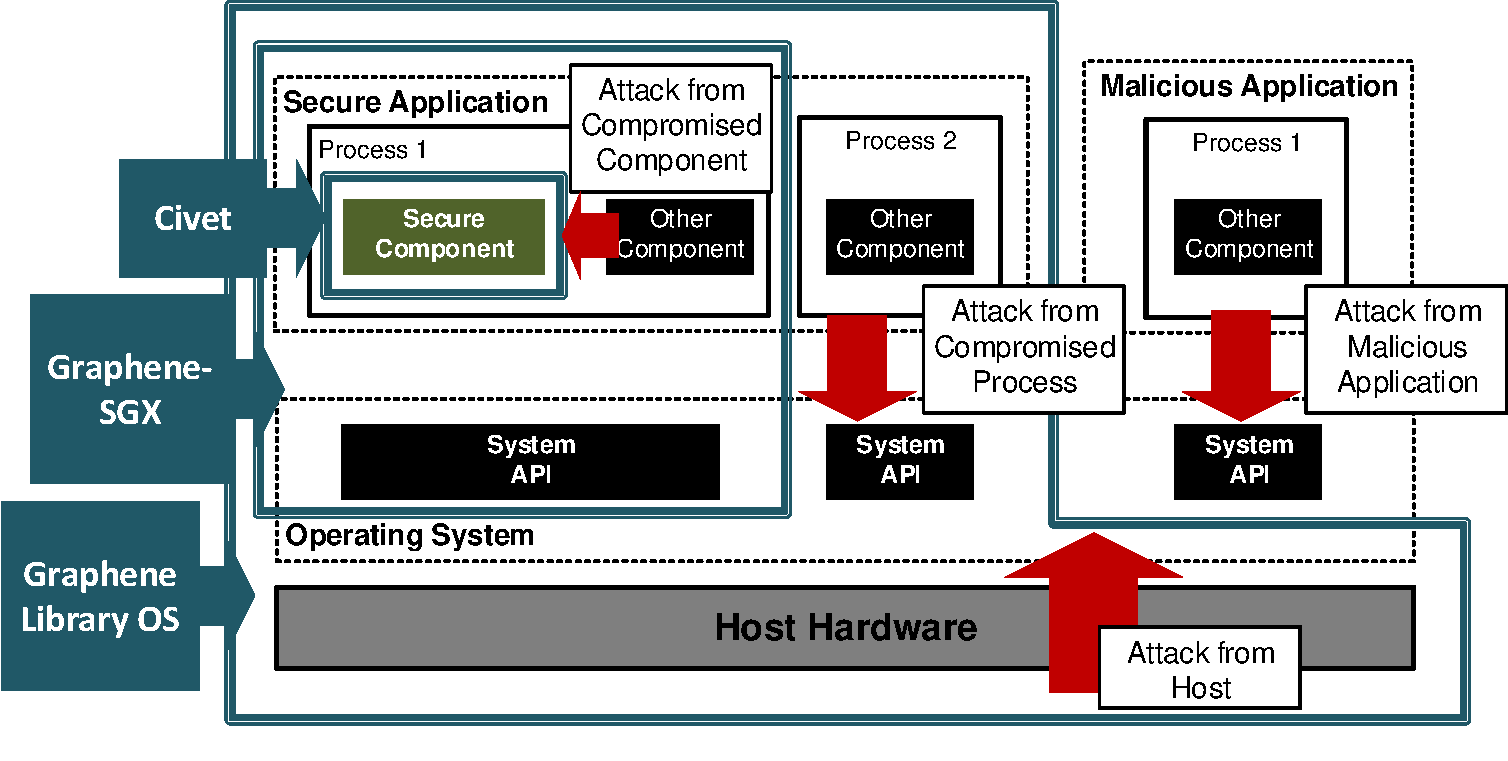
\includegraphics[width=4.5in]{figures/defense.pdf}
%\caption[Types of potential attacks on an application, and the TCB required by \graphene{}, \gsgx{} and \civet{}]
%{Type of potential attacks on the security of an application and the trusted computing base (TCB) required by \graphene{}, \gsgx{} and \civet{}.
%An application can be attacked from either the corrupted host system stack, malicious applications, or compromised components and processes in the application.
%\graphene{} can expel all untrusted applications and the system APIs that are affected by them.
%\gsgx{} further removes the host kernel and hardware, as well as untrusted processes, from the TCB. \civet{} then defends against compromised, in-process components. \graphene{} has the larger TCB, and \civet{} reduces the TCB the most.}
%\label{fig:defense}
%\end{figure}

%This thesis primarily describes three security isolation solutions,
%to defend against different levels of attack (as summarized in Figure~\ref{fig:defense}):
%\begin{compactitem}
%\item {\em \graphene{}} (\S\ref{chap:graphene}) enforces security isolation between mutually untrusting applications.
%\item {\em \gsgx{}} (\S\ref{chap:gsgx}) enforces security isolation on applications against untrusted system stacks and other applications.
%\item {\em \civet{}} (\S\ref{chap:civet}) enforces security isolation inside an application, against untrusted application partitions as well as the system stacks and other applications.
%\end{compactitem}

%\section{Security Isolation for Linux Multi-Process Applications\\ using a Library OS}
%\label{sec:intro:graphene}

%An alternative to virtualization, \emph{\liboses{}}~\cite{porter11drawbridge,unikernels,baumann13bascule}, also emulate OS abstractions in guest-like environments, but have the ability of adjusting the host-guest boundaries, to define suitable host interfaces.
%A \libos{} moves the OS functionality (API components, or \emph{system call tables} in UNIX systems) from a kernel into the application processes, either statically or dynamically linked into a standalone executable. Emulation by \liboses{} provides an undisruptive way of provisioning OS abstraction for applications, on a restricted host platform~\cite{baumann14haven}.
%Using a \libos{} to adopt applications on any operating systems only depends on three prerequisites:
%(1) environment for executing the application,
%(2) minimal host abstractions,
%and (3) emulation of guest OS abstractions.


%This thesis focuses on the \graphene{}~\cite{tsai14graphene}, for justifying the effectiveness of using \liboses{} for OS emulation. The justification of \graphene{} is split into two stages:
%first, defining a host interface portable to many platforms (\emph{Platform Independence}); and, second, building OS emulation that satisfies majority of applications. Using \graphene{}, we show the evidence of running unmodified Linux applications, from the simplest (e.g., a ``Hello World'') to sophisticated ones (e.g., multi-process, server applications).
%The host interface is ported to many platforms, from the most monolithic (e.g., Linux) to the most restricted (e.g., SGX enclaves).
%The \libos{} provides a more reasonable, incremental path of building application support, compared to the open-ended effort needed for emulating OS functionality on individual platforms.
%For every host platforms, \graphene{} simplifies the emulation of a complex modern OS like Linux to a few generic host interfaces such as opening files or creating a clean instance. The rest of emulation effort can be simply inherited from the other host platforms, where \graphene{} is already ported.
%In a nut shell, both virtualization and the \libos{} have reduced most of emulation effort to one-time cost, yet the host interface of \graphene{} is arguably much easier to port, and the scope of porting targets is much broader.
 


%provides a highly portable, \emph{platform independent} platform,
%by splitting the OS functionality from a kernel
%into the application processes.
%%enforce isolation on mutually untrusting process,
%%by essentially \emph{collapsing} OS components
%%into an application library loaded into the user memory of application processes, or \emph{\picoprocs{}}.
%Compared with monolithic kernels,
%\liboses{} minimize the reliance on the correctness or effectiveness of kernels,
%to enforce isolation
%on applications that distrust each other and
%demand a more impenetrable barrier.
%The isolation of \liboses{}
%%The qualitative benefits of \liboses{},
%%including isolating mutually untrusting applications,
%%migrations,
%%and platform independence,
%is based on partitioning the OS instances
%between the mutually untrusting applications,
%and leaving the \liboses{} only a
%narrow, restrictively defined interface to the host kernel.
%%The benefits of using \liboses{} to run applications include
%%isolating %the consequences of having
%%security vulnerabilities in guest OSes,
%%and reducing unnecessary %unneeded or redundant logics causing
%%%performance bottlenecks 
%%overhead for specific \picoprocs{}
%%--- comparable to the benefits of using \emph{virtualization},
%%but at a significantly lower cost.
%%%More recent \liboses{}
%%%provide several qualitative benefits of virtualization,
%%%such as migration and host platform compatibility.
%%%Library OSes move portions of
%%%OS kernel functionality into an application library.
%%%In a \libos{}, the guest OS is 
%%%% dp: too early for this nomenclature, I think
%%% \daniela{(a libraryOS instance)},
%Within a process with a \libos{}, or a \emph{\picoproc{}},
%the \libos{} implements the system APIs (e.g., system calls) and supporting data structures as library functions
%--- mapping the system abstractions and semantics
%to the narrow host interface.
%%a narrow paravirtual interface to the host kernel.
%Recent library OSes improve efficiency over full guest OSes by eliminating duplicated features
%between the guest and host kernel,
%such as the CPU scheduler, or
%%eliminating guest-level multiplexing code, as the library OS supports only one application;
%even compiling out unnecessary guest kernel APIs~\cite{unikernels}.
%Sometimes, on top of a minimized \emph{\microkernel{}} that often has the size and functionality of a hypervisor,
%library OSes or applications can bypass the multiplexing of hardware resource
%to improve the performance~\cite{engler95exokernel},
%or separating system components
%that are intensively shared and bottlenecking the applications,
%such as bulk allocation of processing buffers~\cite{leslie96nemesis}.
%In total, this can reduce the memory requirements of running a single, isolated application
%by orders of magnitude, and similarly
%increase the number of applications which can run
%on a single system~\cite{porter11drawbridge,unikernels}.
%In addition,
%because of the narrowness of host interfaces, % is easier to implement on various platforms
%%than the high-level system APIs,
%the library OSes can be easily ported to an innovative, vastly distinct platform. 
%A typical example is in \emph{\intel{} \sgx{} enclaves},
%where applications are isolated in a restricted environment that is immune to attacks from untrusted host kernel and hardware peripherals.
%A \libos{} can support whole applications in enclaves,
%without expanded attack surface and porting effort on the applications~\cite{baumann14haven}.
%%% dp: This sentence seems a little premature
%%In recent works, library OSes provide rich OS features for isolated contexts while the host OSes are untrusted
%
%%% Library OSes reduce the memory requirements of running a self-contained,
%%% isolated application process
%%% %guest \daniela{I would replaced guest by "isolated process or group of processes (a libOS instance)''}
%%% by orders of magnitude
%%% In a cloud computing environment,
%%% increasing the number of applications per server has enormous
%%% economic benefits.
%%% Even on a desktop or portable system, \libos{}es can reduce the overheads
%%% of sandboxing untrusted code and running applications
%%% designed for another OS.

%Because library OSes execute within a VM \daniela{this phrase does not read good to me because (i) it might imply the picoprocesses need hypervisor support, as misunderstood by reviewer 1 and (ii) you already emphasized the drawbacks of leveraging a VM} or lightweight process ({\em picoprocess}~\cite{xax}),
%library OSes execute with


%The emulation of Linux abstractions in \graphene{} poses several challenges (described in \S\ref{chap:graphene}). Specifically, we identify the key challenge as the Linux \emph{multi-process abstractions}, commonly used in many server-type or shell applications, for job control or splitting executables for modularity and isolation.
%As each application process runs with a singled \libos{} instance, a multi-process application will require multiple \libos{} instances to collaboratively implement an unified OS.
%As platform-specific and delicate these abstraction can be, \graphene{} simplifies the emulation to a general model of distributed OS implementation, using generic, pipe-like RPC streams to coordinate OS states across \libos{} instances.
%The multi-process abstractions emulated by \graphene{} include forking, {\tt execve}, signals, System V IPC, file descriptor sharing, exit notification, etc.
%\graphene{} emulates these abstractions without introducing any platform-specific host features, including memory sharing, except an optional bulk IPC feature purely for optimization.

%Legacy application support is provided
%in recent \liboses{}~\cite{porter11drawbridge, baumann13bascule, baumann14haven},
%%, such as Drawbridge~\cite{porter11drawbridge}, Bascule~\cite{baumann13bascule} and Haven~\cite{baumann14haven},
%%partial support for legacy applications is provided
%by emulating the OS personalities in individual \picoprocs{}.
%Among the OS abstractions and features that need to be emulated,
%the emulation of
%single-process abstractions,
%such as accessing unshared files, or creating multiple threads in a process,
%can be wrapped inside
%a \picoproc{}, %, with proper level of translation and bookkeeping.
%thus often relatively straightforward.
%For instance, %Drawbridge loads legacy Windows applications including Microsoft Word.
%Drawbridge~\cite{porter11drawbridge} provides Windows abstractions and personalities,
%with 5.6 million lines of code reused from Windows 7
%to emulate the complete OS personality in a single \picoproc{},
%except a few features such as the Windows registry that has to be implemented
%separately as in-process libraries or services.
%%using in-process services. % such as the Windows registry.
%However, when it comes to emulating multi-process abstractions,
%%in contrast to single-process abstractions,
%%multi-process abstractions 
%which are commonly used by Unix applications,
%%are more challenging, % to emulate in \picoprocs{},
%%due to the assumption and
%%narrowed interfaces of \picoprocs{}.
%\picoprocs{} serving multiple processes of an application
%will need to collaboratively provide shareable OS abstractions,
%and more importantly, a unified OS view to the application.
%%% dp: Daniela, great suggestion!  We need to make this situation seem more
%%%     like the sky will fall without our help
%%A key drawback of recent library OSes, however,
%%is that they are limited to single-process applications.
%%Yet many applications, such as network servers and
%%shell scripts,
%%create multiple processes
%%for
%%performance scalability, fault isolation, and programmer convenience.
%%These applications would benefit from the efficiency and security benefits
%%of a library OS.
%%In order for the efficiency benefits of \liboses{} to be widely applicable,
%%especially for unmodified Unix applications,
%%either applications must be rewritten to implement ad hoc coordination mechanisms, or
%%\liboses{} must provide commonly-used multi-process abstractions,
%The multi-process abstractions to be emulated include
%forking, signals, System V IPC, file descriptor sharing, exit notification, etc.
%A possible alternative is
%%To support multi-process abstractions, \liboses{} often have 
%to rely on %sharing OS states,
%the hosts' memory sharing features to share OS states.
%However, memory sharing is not always an available features in the host:
%for example, Drawbridge and Bascule~\cite{baumann13bascule} cannot emulate process forking because copy-on-write memory sharing is not a platform-independent features.
%Furthermore, when Haven isolates applications
%in enclaves,
%memory sharing is strictly forbidden by the hardware platform,
%to prevent leaking secret to other enclaves.
%In a word, emulating OS abstractions and personalities can fundamentally
%oppose the assumptions or limitations of the system,
%causing obstacles to supporting legacy applications.



%The purpose of \graphene{} is more than benefiting the platforms where the host interfaces are fully ported.
%Even when the host interface is only partially implemented,
%\graphene{} provides a way for system developers to estimate and reason about the completeness of emulation.
%For example, allocation and assignment of thread-local storage based on x86 segment registers ({\tt FS}/{\tt GS})
%is natively required in most Linux applications.
%We observe that, as some host platforms (e.g., Win32 and OSX) may confiscate the segment registers for their own reasons,
%implementing this host interface ({\tt DkSegmentRegisterSet}) is not necessary feasible on every platforms.
%Instead of obligating full compatibility,
%\graphene{} allows the host platforms to skip host interfaces,
%while the developers can determine or even measure the consequence (the measurement model is described in \S\ref{chap:syspop})---such as asserting the applications that are not supported.
%Moreover, for specific interfaces,
%the \libos{} can even provide generalizable, platform-independent workarounds to address the portability problem,
%with acceptable penalty on performance.


%\begin{figure}[t!]
%\centering
%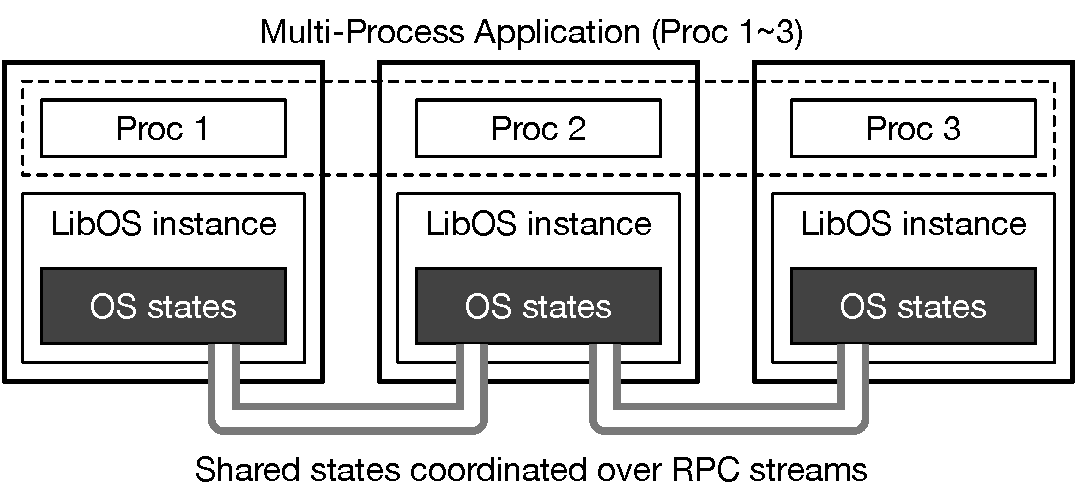
\includegraphics[width=0.75\linewidth]{graphene/figures/concept.pdf}
%\caption[Multi-process abstraction model of \graphene{} \libos{}]
%{Multi-process abstraction model of \graphene{} \libos{}. For each process of an application, a libOS instance will serve system calls and keep local OS states. States of multi-process abstractions are shared by coordinating over host-provided RPC streams, creating an illusion of running in single OS for the application.}
%%\vspace{-.1in}
%\label{fig:graphene:concept}
%\end{figure}

%We present {\em \graphene{}}, a Linux-compatible \libos{} to secure unmodified, Linux multi-process applications.
%In \graphene{}, multiple \libos{} instances collaboratively implement
%multi-process abstractions,
%yet appear to the application
%as a single, shared OS.
%\graphene{} instances coordinate state using remote procedure calls (RPCs) over
%host-provided, pipe-like streams.
%In a distributed POSIX implementation, placement of shared state and messaging complexity
%are first-order performance concerns.
%%We chose to shift implementation complexity into the library OS
%%in order to uphold simple enforcement of security isolation in the host.
%By coordinating shared states across \libos{} \picoprocs{,
%\graphene{} is able to create an illusion 
%of running in a single OS
%for multiple processes in an application.

%Previous library OS designs ensured security isolation of independent applications,
%comparable to a VM, by keeping a relatively narrow host ABI.
%We selected the \graphene{}
%design because it strikes a unique balance between
%and robust, flexible security enforcement.

%The design of \graphene{} ensures security isolation of
%mutually untrusting, multi-process
%applications on the same host.
%Essential to this goal is
%minimally expanding the host ABI to support multi-processing,
%as well as leveraging RPCs as a natural point to mediate inter-\libos{} communication.
%RPC coordination among \graphene{} instances can be dynamically disconnected, facilitating novel sandboxing
%techniques.  For instance, we develop an Apache web server extension that, upon logging in a given user,
%places the worker process's \libos{} in a sandbox with access to only that user's data.
%We expect more nuanced degrees of trust are possible in future work.

%\graphene{}'s design gives the user and system administrator a high degree of flexibility
%in isolating arbitrary groups of unmodified application processes,
%while upholding the efficiency and host compatibility benefits of recent \liboses{}.


%The key to emulating multi-process abstractions in a \libos{},
%especially when memory sharing is not safe or available,
%is to coordinate shared OS states
%across \picoprocs{} using limited host abstractions.
%%The \libos{} of related \picoprocs{} %that accompany application processes
%%must collaboratively provide a unified OS view
%%to the application.
%The OS states needed to be coordinated
%are primarily in three types:
%process states that are inherited at process creation
%(e.g., {\tt fork}, {\tt execve});
%abstraction states that are shared among related processes
%(e.g., signals, \sysvipc{} semaphores);
%and namespace states to locate the owners of abstractions
%(e.g., process IDs, \sysvipc{} keys).
%A \libos{} that implements all the idiosyncratic OS states
%must not overly expand the host interface,
%and compromise the security isolation or platform independence of the system.
%%and thus increase the risk of
%%allowing malicious applications to compromise the host kernel.
%As a solution, we present \emph{\graphene{}},
%a Linux-compatible \libos{} that collaboratively implement
%various Linux multi-process abstractions,
%yet appear to the application as a single, shared OS.
%\graphene{} instances coordinate all OS states using remote procedure calls (RPCs) over
%host-provided, pipe-like streams.
%The use of host RPC streams
%does not expand the host interface already used by a single \picoproc{},
%and can be naturally isolated
%by sandboxing the RPC streams from the host.
%%with the application.
%%In a distributed POSIX implementation, placement of shared state and messaging complexity
%%are first-order performance concerns.
%%%We chose to shift implementation complexity into the library OS
%%%in order to uphold simple enforcement of security isolation in the host.


%\fixmedp{After a complete draft is written, coalesce all goals and make sure they are addressed early on.  We are doing some scatter-shot motivation}

%\section{Isolating Native Applications on Untrusted Hosts}
%\label{sec:intro:gsgx}

%The complexity of modern operating systems has become
%a major source of security vulnerabilities,
%pressuring developers to seek solutions to exclude the host OSes
%from their trust models.
%The untrustworthiness of OSes get severe when applications are run in the cloud,
%because the applications may cohabit with compromised tenants,
%or be hosted by malicious providers.

%Existing works provide isolated execution of applications
%on untrusted operating systems or host hardware,
%using either hypervisors~\cite{criswell2014virtualghost, flicker, inktag, zhang2012mushi} or security hardware~\cite{intelsgx, secureblue++}.
%Especially security hardware such as \intel{} \sgx{}~\cite{intelsgx} can defense against hardware-level attacks,
%with low execution overhead.
%\sgx{} is a set of new instructions introduced in the latest \intel{} CPUs,
%to create a encrypted memory region called {\it enclave}
%in the application's address space.
%\sgx{} guarantees that only signed code loaded in the enclave can access the sensitive data stored in the enclave memory.

%Protecting applications without the requirement of trusting the hosts
%has become valuable in modern computer systems for many reasons.
%The complexity of the existing commodity operating systems has become a major source of
%vulnerabilities to exploit.
%Once the host operating systems are compromised,
%any security mechanisms enforced in the applications can be easily circumvented.
%If the applications run in the cloud,
%the hosts have to be controlled by the cloud providers,
%which is capable of compromising both host operating systems and hardwares.
%The attacks from the cloud is possible even if
%the operating systems' vulnerabilities are never exploited.

%However, isolating an application with \sgx{} enclaves
%requires additional porting effort,
%to partition the application into a signed, trusted binary,
%and the rest.
%Only the trusted binary will be loaded in enclaves.
%The enclave will interact with the rest of the application
%through an {\em untrusted interface},
%to pass input and output of the isolated execution,
%and access OS features such as files and network.
%For a complex application such as a network server or a desktop GUI,
%the effort to partition the application is too high,
%and the untrusted interface is often too large,
%given the complexity of interaction between the enclave and the rest of the application.

%Unfortunately, leveraging SGX for security
%often requires rewriting the applications to a large extent.
%Because the OSes cannot be trusted,
%enclaves are not allowed to directly access any system interface
%for any OS features
%such as files, networks or scheduling.
%Only a limited subset of system library API can be exported in enclaves;
%for example, the software development kit for SGX
%only supports spin-locking as scheduling tool,
%because other primitives require cooperation from the OS.


%With the support of a \libos{}, developers can port an application to \sgx{} with minimal effort,
%using a {\em non-partitioned model}~\cite{baumann14haven}.
%The non-partitioned model loads the whole application binary into the enclave,
%and a \libos{} to support the OS features.
%The benefits of using a non-partitioned model also include
%limiting the untrusted interface to a narrow, fixed interface,
%and the fact that the application is protected ``as is''
%--- especially useful for privacy-preserving applications.


%In particular, the platform independence of \liboses{}
%allows porting legacy applications to platforms with more restricted interfaces
%and functionalities than monolithic kernels,
%such as \intel{} \sgx{} enclaves.
%The essence of isolating applications using \liboses{} in enclaves
%is to ensure
%the security benefits promised by the platform,
%%in an system enforcing stronger security isolation
%%on legacy applications,
%%such as Haven~\cite{baumann14haven},
%%it is necessary
%%%the system must not only emulate the personalities,
%%to provide the security benefits promised by the platform
%%(i.e., enclaves).
%%%instead of simply emulating the personalities.
%%For instance,
%%the security benefits of enclaves
%including application integrity,
%sealing confidential information,
%and attestation.
%%These benefits must be also provided by systems that use enclaves to isolate legacy applications.
%An existing system, Haven~\cite{baumann14haven},
%packs a Windows-compatible \picoproc{}
%into an enclave,
%using an encrypted virtual disk
%securely provisioned from a remote, attested server.
%Haven essentially provides a trusted path to safely load application and \libos{} binaries,
%as well as mediating all input and output to the host.
%%as the trusted path to safely load application and \libos{} binaries.
%%Haven relies on
%%%the \libos{} to
%%securely provisioning an encrypted virtual disk
%%from a trusted, remote server,
%%to ensure a \emph{trusted path} to
%%load authenticated application binaries
%%and redirecting IOs,
%%yet appears
%%completely transparent to the application.
%The only limitations in the model of Haven, however, 
%%are the huge TCB (trusted computing base)
%%caused by the \libos{} (209MB in total),
%are the lack of multi-process support,
%and being overly reliant on the remote server.
%% and being incapable of isolating multi-process applications.
%% especially in the finer, per-process granularity.
%Addressing these issues,
%by porting \graphene{} to enclaves
%(\emph{\graphenesgx{}}),
%we reassure multi-process, UNIX applications in a multi-enclave environment.
%The application integrity in \graphenesgx{} 
%is validated on unencrypted,
%regularly distributed binaries,
%using checksums
%signed by the hardware-attested measurement
%--- an off-line model without relying on
%remote servers.
%\graphenesgx{} ensures that
%process creation in enclaves can be scalable, and individually configured
%--- a parent enclave can identify and restrict
%the application binaries to be loaded into any child enclaves it creates.
%%to isolate multi-process applications in a multi-enclave environment.
%%The coordination of \graphene{} based on RPC streams
%%allows isolated \picoprocs{} to build a trusted path for OS coordination,
%%by attesting and encrypting the RPC streams.
%%\graphene{} verifies binary integrity using per-binary checksums,
%%to rid most application behaviors
%%of the dependency on remote trusted servers,
%%and to allow each \picoprocs{} be attested and provisioned individually.
%
%
%
%%To alleviate the pain of migrating applications to SGX,
%%recent works like Haven~\cite{baumann14haven} provides a mechanism
%%of loading native applications into enclaves,
%%alongside a library OS to facilitate rich OS features.
%%These systems are called ``shielding %systems''~\cite{xu15controlledchannel},
%%which means these systems can secure execution environments
%%without trusting the host.
%
%%A primary drawback of the non-partitioned model is the huge TCB loaded into the enclave.
%%In the partitioned model, only minimal code needed for the isolated execution will be loaded into the enclave.
%%However, in the non-partitioned model, the whole application must be loaded into the enclave,
%%in addition to the TCB contributed by the \libos{}.
%%For instance, size of the \libos{} used in \cite{baumann14haven} is 209MB,
%%which yields significant expansion to the original TCB.
%%
%%We present {\em \gsgx{}}, a port of \graphene{} \libos{} on \sgx{}, to secure unmodified Linux applications in \sgx{} enclaves{}.
%%The support for Linux applications
%%has been missing in the non-partitioned model,
%%which is a missed opportunity according to the 75\% market share of Linux cloud providers~\cite{linuxcloud2014}.
%%\gsgx{} supports most OS features provided by \graphene{}
%%including both single- and multi-process abstractions.
%%
%%The design of \gsgx{} ensures the minimal enclave TCB
%%that can be achieved without further partitioning any application binaries.
%%The integrity of the loaded application binaries
%%is enforced in a fine-grained fashion:
%%each binary must be signed and checked individually,
%%and only binaries that are actually needed will be ever loaded.
%%For multi-process applications,
%%\gsgx{} isolates each \picoproc{} in a separate enclave,
%%thus every \picoproc{} can execute and be attested separately.
%%In a nutshell, \gsgx{} tries to honor and exploit the established partitioning in multi-process applications,
%%with the benefit of minimizing the porting effort from using the non-partitioned model.
%
%
%\paragraph{Improving Efficiency with Legacy Support.}
%One of the other first-order requirements in systems, besides legacy support,
%is to pursue low latency or high throughput,
%according to how users define quality of service.
%Nevertheless, there is a trade-off between the emulation of OS personality
%and the efficiency of system operations.
%\graphene{}, for instance, coordinates OS states %for multi-process abstractions
%over PRC streams,
%and requires strategies to mitigate the significant RPC coordination overhead.
%%will cause nonnegligible overhead to the latency of IPC,
%%in comparison with coordination by memory sharing. % in the kernel or in the \picoprocs{}.
%%However, when designing a \libos{},
%We observe, in a distributed UNIX implementation,
%placement of shared OS states and
%messaging complexity
%are essentially the top performance factors.
%%%there are opportunities to identify and remove unneeded or redundant
%%%overhead or bottleneck,
%%%especially on the critical or common paths.
%%%%frequent operations.
%%%An example of reducing overhead
%%%is to remove redundant permission checks in \liboses{},
%%%because \picoprocs{} rely on the host kernel to enforce security policies.
%%%Similarly, to compensate the overhead of IPC
%%%in a distributed implementation, placement of shared OS states and messaging complexity
%%%will be the first-order performance concerns.
%%For \picoprocs{} that most frequently access an abstraction state,
%%place the state in this very \picoproc{}
%%will optimally avoid the need for coordination over RPC streams.
%Improving the coordination overhead will require placing the OS states in the most frequency accessing \picoprocs{},
%and reducing round trips of RPC messages.
%
%\paragraph{Partitioning Legacy Applications.}
%Beside supporting whole applications,
%%and derive principles to improve the result of implementation.
%we also explore the opportunity of partitioning a legacy application,
%in a model where it is split into
%trusted and untrusted components that are isolated by platforms like enclaves.
%The partitioned model for porting to enclaves
%is commonly used for quarantining the extremely sensitive execution
%in an application.
%The purpose of partitioning is to
%defend against the whole, untrusted host systems (except the CPUs)
%as well as other less sensitive components,
%in order to minimize the trusted computing base.
%The weakness of the model is,
%partitioning an application requires additional effort to identify and separate
%the execution that needs to be protected,
%and the effort becomes unacceptably expensive when the application is considerably sophisticated.
%In particular, we are targeting applications implemented
%in a managed language such as \java{},
%which are more likely to be automatically compartmentalized
%using programming language techniques.
%
%
%%We observe that in order to partition a system or application
%%in finer granularity,
%%%such as an extremely sensitive component,
%%%legacy code reuse will become even more challenging.
%%%In this case,
%%%inevitably,
%%applying techniques from programming languages %and code analysis
%%will become necessary.
%%Specifically, one technique that developers will need is automated compartmentalization of legacy code.
%%%The reason is, 
%%Unless the partitioned component code is compact and simple,
%%the effort required
%%for cleanly and minimally partitioning the code
%%will be too high.
%%For an application developed in a managed or object-oriented language (e.g., \java{}),
%%code compartmentalization can be effective enough to create close-to-optimal partitioning.
%
%The motivation for pursuing \java{} application partitioning
%is two-folded.
%On one hand,
%many enterprise or cross-platform applications
%are developed in \java{},
%but so far no enclave support for whole or partial \java{} applications
%is ever provided.
%%To load an application into an enclave,
%%both the execution and interface of the application code
%%have to be static
%%ever since the enclave starts.
%%Because \java{} classes are dynamically loaded and managed by \java{} VMs,
%%extra support from the system will be necessary.
%On the other hand,
%execution isolated in an enclave must be unconditionally trusted;
%if any vulnerabilities exist in the execution,
%the attack can infiltrate from the untrusted host to compromise the isolation.
%However,
%just as the whole application,
%the isolated part is also hard to completely eliminate vulnerabilities.
%%an application or component isolated in an enclave must be %verified to
%%immune to security vulnerabilities,
%%otherwise there will be risks of leaking the enclave secrets.
%By allowing developers to port \java{} applications into enclaves,
%protection mechanisms based on
%the characteristics of \java{} language,
%such as type checking, information flow tracking among objects,
%can further ensure the soundness of isolated execution.
%The automated partitioning of \java{} applications into enclaves
%is an ongoing work.
%
%
%%
%%Haven effectively migrates native Windows applications to enclaves,
%%providing a shortcut for developers
%%to easily boost the security of their products.
%%However, there are several limitations in Haven, including
%%excessive trusted computing base (TCB),
%%a restrictive model of adapting applications,
%%and missing support for Linux or multi-process applications.
%
%%We present \gsgx{}, a \libos{}-based shielding system
%%targeting Linux multi-process applications,
%%as improvement to the Haven model of migrating native application to SGX.
%%\gsgx{} is derived of \graphene{}~\cite{tsai14graphene},
%%which supports 139 out of 300 Linux system calls.
%%\graphene{} runs numbers of popular applications
%%such as Apache web server, OpenJDK virtual machine, or shell scripts,
%%all of which relies on multi-process abstractions
%%such as {\tt fork}, {\tt execve}, signals or System V IPC.
%
%
%
%
%\paragraph{Measurements for System Completeness.}
%In general, due to the complexity of implementation or preserving
%the complete specifications,
%developers must prioritize the development based on
%what they believe to be more important
%--- what will impact or satisfy more applications or more users.
%Especially for innovative systems like \liboses{},
%developers struggle to evaluate the progress in a partial prototype.
%%From improving legacy code compatibility in different systems
%%(Linux to \graphene{}),
%%we observe that system developers including us
%%routinely make design choices based on 
%%what they believe to be the common and uncommon behaviors of a system.
%%For instance, in \graphene{}, we start with handpicking the abstractions and specifications
%%that we believe to be more important to the applications.
%%When optimizing Linux file system directory cache,
%%we shorten the latency of {\tt stat} and {\tt open} system calls
%%at the expense of {\tt rename} and {\tt chmod},
%%assuming that {\tt stat} and {\tt open} are the more commonly used operations in majority of applications.
%%%In the case of a general-purpose OS, determining
%%%exactly what the common case is can be challenging.
%%In general,
%%a developer's view of what system APIs are important is skewed towards
%%the developer's preferred workloads.
%%%the choice of what features matter skews heavily towards
%%%workloads particular developers use.
%%Similarly, developers who struggle to evaluate the impact of a 
%%change on compatibility
%%must implement every abstractions and specifications,
%%and then be able to reason about the completeness of legacy support.
%%support of legacy application in the product system.
%At the center of these problems is the missing of information about how system abstractions or APIs are used in the run-time.
%%and a metric to estimate the completeness of legacy applications that can be supported
%%for any random users.
%In search of better methods for
%evaluating the legacy support,
%we conduct a study of Linux system APIs usage among a large sample of Debian/Ubuntu x86\_64 applications,
%weighted by the application popularity
%collected by the Popularity Contests~\cite{debian-popularity, ubuntu-popularity}.
%Based on the study,
%we create a measurement
%for estimating the fraction of applications installed by a user
%that can plausibly use the system.
%For instance, the current \graphene{} prototype,
%in which we hand-pick Linux system calls according to the applications for experiment,
%can support the complete API footprint
%in 0.42\% of applications installed by a user.
%The data-driven, principled strategy shows than \graphene{} can be improved to
%supporting 21.1\% of applications,
%by simply adding two missing system calls, {\tt sched\_setcheduler} and {\tt sched\_setparam}.
%
%%We create sensible, representative metrics,
%%which measure the effects of both applications and users.
%%Using the metrics and insights from the study,
%%the significant improvement on legacy application support in \graphene{} is demonstrated
%%if we guide the development using this approach.
%
%%Summarizing all contributions of the thesis,
%%we explore the solutions and principles,
%%to implement OS support for legacy applications in either 
%%isolated systems
%%(i.e., \graphene{} \libos{}, enclaves) 
%%or optimized legacy OS components
%%(i.e., Linux file system directory cache).






%By supporting Linux multi-process applications,
%\gsgx{} simply applies to a broader range of cloud-based applications
%than Haven.
%Survey shows that Linux yields a market share of up to 75 percent in
%enterprise cloud providers~\cite{linuxcloud2014}.
%This data suggests majority of the existing cloud users can
%more easily adopt \gsgx{} than Haven.

%\gsgx{} uses a different model from Haven
%to bootstrap the trust of loaded applications.
%Haven builds up the trust by packing all binaries
%in an encrypted virtual disk,
%with secret key provisioned consensually from a remote server
%trusted by the clients.
%Contrastingly, \gsgx{} relies on a model directly derived from
%the trust model of \sgx{},
%by including applications' checksums
%into the enclave measurement to be attested by hardware.
%\gsgx{} can migration applications for enclaves off-line,
%and share binaries (e.g., shared libraries) to save bandwidths for deployment.
%
%Security-wise speaking,
%\gsgx{} provides a way to reduce the TCB of enclaves,
%with a smaller code footprint
%and applications natively partitioned as processes.
%Haven in general yields a large TCB
%including a \libos{} as large as 209MB,
%and application binaries around 10s \textasciitilde 100s of MB.
%The image of \gsgx{} is merely 10MB,
%and Linux applications generally follow the principle of dividing
%code into smaller, more testable binaries.
%\gsgx{} isolates multiple binaries (or processes) of an application
%in separate enclaves, and authenticates inter-process coordination
%by binary-based policies.
%Even if an enclave is compromised, other enclaves of the same application
%can still stay secure as long as
%critical information never flows to the victim.
%
%\gsgx{} provides cloud users
%ease of shielding Linux applications
%and flexibility of implementing any desired security model
%suitable for each binary.

%\section{Combining Isolated Execution with Language Protection\\ for Partitioned Applications}
%\label{sec:intro:civet}

%% \fixme{Chia-Che Tsai's opening}
%% Modern security hardwares such as TPM or \sgx{}
%% provide hardware enforced guarantees of security properties
%% even upon %untrustworthy hosts with
%% compromised operating systems or tampered hardwares.
%% The reasoning of security using these hardwares
%% is often founded as follows:
%% An untamperable hardware package such as CPU will guarantee
%% the integrity of applications loaded
%% exactly identical to the images signed by clients.
%% However, to achieve overall security,
%% the clients are still responsible for ensuring that no vulnerabilities
%% within the signed images
%% will compromise the security properties in runtime.

%%\fixmedp{I would start by motivating the goal of application partitioning.
%%I think you could add a little more here, but this is a rough sketch.}
%For applications that handle sensitive data such as private keys,
%or implement proprietary algorithms,
%running on a untrusted host whose hardware and hypervisor
%may be compromised is a huge risk.
%%, such as medical applications, or 
%%implement proprietary algorithms, such as algorithmic stock trading.  
%%These applications are composed of 
%%libraries and other code from third parties, and may run on 
%%hardware and hypervisors provided by an untrusted cloud provider.
%%Using the partitioned model the developers can 
%%bound the effort to protect sensitive data and algorithms,
%%while still taking advantage of inexpensive code and cloud hardware.
%%A partitioned application isolates sensitive data and code, typically using
%%language or hardware techniques.
%If users run these applications in isolated execution such as \sgx{},
%due to the complexity of the applications,
%the cost of partitioning and porting the applications may be too high to pay.
%However, as discussed in \S\ref{sec:intro:gsgx},
%using the non-partitioned model, the application must tolerate a much larger TCB in the isolated execution,
%whereas a large fraction of the TCB is less sensitive.
%
%A solution to this dilemma
%is to automate the partitioning using language techniques.
%For instance, applications implemented in managed languages like \java{}
%are easier to partition,
%if a few hints about the sensitive data can be provided by the developers.
%Since \java{} classes are often well modularized,
%an automated language-level tool can analyze the minimal supporting classes to process the sensitive data,
%creating a clean partition with more reasonable TCB.

%%Why SGX
%%\fixme{Bhushan's opening}
%At the hardware level, 
%new CPUs are offering features to protect application-level code and data
%from a  compromised or malicious system software stack,
%including the OS or hypervisor, or simply isolating portions of the 
%application address space from the rest of the application.
%Examples include SX~\cite{sgx-manual}, 
%%\fixmedp{Can we mention/cite others? IBM and ARM?}
%IBM SecureBlue++~\cite{secureblue++}, and ARM TrustZone~\cite{trustzone}.
%%are offering models of mutual distrust, which facilitate protecting
%%an application from a
%SGX offers %One feature of SGX is restricted
%entry points to an encrypted region of memory, called an {\em enclave}.
%Encryption and remote attestation 
%prevent the hypervisor or OS from reading or modifying the enclave's contents,
%and validate that the enclave was correctly initialized.
%This in turn
%can exclude 
%a cloud provider's hypervisor or OS from the application's trusted computing base (TCB),
%requiring only trust in the hardware manufacturer (i.e., Intel).
%%Remote attestation can also validate that an enclave was correctly initialized.
%%Enclaves also provide remote attestation, where a client
%%can ascertain whether the hardware is genuine Intel, and that the application was
%%loaded correctly.
%SGX also offers protection against malicious devices off the CPU package,
%such as a compromised storage device.


%Besides automated partitioning,
%securing \java{} applications in \sgx{} opens opportunities to hardening the security of isolated execution,
%using language-level protections
%~\cite{bittau2008wedge,brumley2004privtrans,khatiwala2006data}.
%For instance, the type-checking feature in the \java{} language
%can avoid the risk of exploitable pointers or control flow errors,
%which is significant in an unsafe language like C
%~\cite{nergal2001libc,bletsch2011jump,checkoway2010return}.
%
%In addition, although SGX can restrict enclave entry 
%to a few predefined entry points,
%the developers still have to reason about what the soundness of the
%entry-point definitions, protection against malicious inputs,
%and the code paths that must not inadvertently leak sensitive data.
%For instance, Iago attacks~\cite{checkoway13iago}, where an OS offers malicious system call return values,
%can be notoriously difficult to defend against from an enclave;
%although limited countermeasures exist for the OS API (typically with the cooperation of a 
%trusted hypervisor)~\cite{kwon2016sego},%\fixmedp{cite the asplos 16 inktag paper},
%there are no off-the-shelf defenses against Iago-style attacks from the compromised application code.

%Further, SGX is designed to run a small, native code library inside of a larger
%application; support for running managed languages in an enclave is currently limited.  
%Writing a security-sensitive application in an unsafe
%language like C dramatically increases the risk of exploitable pointer or control flow errors, which ultimately disclose sensitive data or undermine the integrity of the enclave.

%Modern security hardware
%such as  provides hardware protection to applications
%especially the ones deployed in the cloud,
%so that the applications do not have to trust the privileged
%OS layer controlled by the cloud provider. 
%against malicious system stacks, including OS, hypervisors or devices. 
%In principle, these hardware techniques 
%Hardware protection between applications and their hosts is appealing
%in cloud computing, because the cloud client 
%need only trust the 
%the cloud provider's hypervisor can, in principle, 
%be excluded from the application's trusted computing base (TCB).
%These hardware protection is especially essential for cloud computing, due to the multi-tenant environment and potentially compromisable providers.
%\fixme{I want to emphasize it can defend against hardware attack.}
%This type of hardware creates a sanctuary for the most security-sensitive
%components of an application---

%For instance, SGX creates a encrypted memory region 
%called {\em enclave} within the memory space of an application,
%which can only be accessed by verified code from the users.
%\fixme{I rather not emphasize partitioning so early, it's not the only way of using enclave.}
%SGX lets the developer partition the application into two parts --- 
%security sensitive and non-security sensitive parts. The security
%sensitive part of the application is run in an hardware isolated
%sandbox called enclave, while the non-security sensitive part runs
%normally outside the enclave.
%% SGX guarantees not only the integrity of loaded application image,
%% but also the confidentiality
%% of application data, %in enclave,
%% avoiding any information leakage to the untrusted exterior world.
%SGX provides a fail-safe way to prevent information leakage from the enclave:
%by guaranteeing the integrity of a measured %and verified
%application binary
%and the confidentiality of application data in memory.
%the OS or hypervisor are simply stopped from peeking any application data, unless the isolated applications release any information. 

%Language-level techniques can offer more sophisticated insights into how
%to partition the application, as well as stronger protections ~\cite{bittau2008wedge,brumley2004privtrans,khatiwala2006data}.
%%\fixmedp{Can we bless some language-level app partitioning tools here?}
%Similarly, managed languages such as Java, with type-checking,
%can prevent memory corruption attacks,
%while applications developed in C or C++ are often prone to memory-bug exploitation.  
%Because Java is memory safe, it is immune to known control flow attacks, such as return-oriented programming,
%where control flow is manipulated by unsafe writes to return pointers on the stack or function pointers in objects.

%protection prevents applications from being compromised by
%vulnerabilities that exist inside the applications.
%The vulnerabilities include mistakes made by developers, such as semantic and configuration bugs,
%and unbound application behaviors that can be exploited by attackers,
%such as memory attacks or control flow attacks.
%Based on the different languages used by developers,
%applications can be offered stronger language specific security guarantees.

%Although combining isolated execution and language protections
%is beneficial for partitioned applications,
%the synthesization of the two mechanism can be difficult in practice.
%%In general, hardware protection and language-level protection 
%%provide separate security guarantees.
%%Unfortunately, developers often struggle to combine both types of protection, due to the limitations and lack of support for both approaches.
%We focus on the combination of \sgx{} and \java{} as a running example:
%\sgx{} are designed to run native code that is primarily developed in C or C++.
%Without further support, a partitioned \java{} application
%cannot be directly loaded into an enclave.
%There is also no API support for \sgx{} features in \java{},
%making it challenging for \java{} applications to use any \sgx{} features to their advantage.
%%Developers often have to create an ad hoc integration of hardware and language-level protection,
%%or they are forced to exclusively expose the application between
%%attacks from the system stacks and vulnerabilities inside the applications.
%The current state-of-the-art of secure more complex applications with \sgx{} is to develop ad hoc solutions that target specific use cases.
%% approaches of combining
%%language and hardware protection often rely on ad-hoc solutions that
%%are specific to certain use cases or technologies.
%For example, \cite{vc3} use \sgx{} to secure data analysis in a MapReduce framework supporting C++
%--- instead of the Hadoop framework that generally supports \java{}.

%% dp: this sentence seems off track, unless you want to say something about ``this has to be in C''
%Similarly, S-NFV uses SGX to isolate states of Network Function Virtualization Applications~\cite{shih2016s}.

%\fixmedp{Please check the previous 2 sentences for accuracy; if I'm wrong, try to say something more crisp.
%Also, any other important related work here?}
%to utilize SGX hardware in language runtimes,
%a set of APIs may be exported through the native interface to support certain high-demand use cases, such as Hadoop workloads
%Although these existing solutions nicely support a part of the users,
%and potentially have demonstrated some common wisdom for combining the language and hardware protection,
%the problem of how to generalize the approach
%to cover more use cases or technologies that the authors haven't forseen,
%still remains unsolved.

%% dp: This paragraph is a little too much philosophy for me.  Cutting for now, but can bring some fo this back later in the intro if needed.  I think it would be better for explaining the benfits of Civet.
\begin{comment}
We use SGX vs Java-based protection as an example,
to show how the guarantees ({\em what is secured?})
and features ({\em how is it secured?}) of hardware protection
can be properly modeled at the language level,
so that language protection mechanisms can be extended
to mitigate vulnerabilities in hardware protection. 
For instance,
SGX hardware provides isolation between multiple
levels of security sensitivity in an application process,
by building another privilege level that bypasses the OS or hypervisor.
We model this hardware guarantee at language level by asking the developers
to identify the multi-level security sensitivity in the application.
The developers do not have to worry about
when to enter or leave the enclaves,
what information to flow out of the enclaves,
or even how SGX enclaves fundamentally work.
The language features
such as implicit and explicit information flow tracking can be {\em leveraged}
by the low-level component that interfaces with SGX enclaves
as the criterion for whether certain information
is safe to be released from the enclave.
\end{comment}
%while 
%


%to the privileged
%or un-privileged code outside the \enclave{}.

%One of the primary concerns on the security of enclaves is
%the strong assumption
%that enclaves' security guarantees rely on---
%The security guarantees of hardwares like SGX rely on a strong assumption:
%To provide the confidentiality guarantees,
%the code running in an enclave must not
%the secured environment (\enclave{}) must not
%have %any bugs or
%vulnerabilities that can be exploited for causing any information leakage.
%However, without language support, it is hard to ensure that
%the enclave code is
%free of vulnerabilities, especially if written in C---which provide no memory safety.
%the SGX only supports programs 
%written in C or C++, and it is extremely difficult to find
%all the memory corruption bugs in the enclave code written in C or C++.
%Without memory safety, 
%the control flow of the code %within the enclave
%can be manipulated by exploiting memory corruption.
%This type of vulnerabilities will lead to information leakage,
%defeating the purpose of using SGX enclaves.
%secure hardware such as
%SGX in the first place. 


%% Lack of memory safety using C or C++ in SGX-secured environments \fixme{maybe spell out why it's hard for SGX}
%% enervates any software approaches to reinforce application security, including control flow and information flow integrity, 
%% %These memory corruption bugs can be exploited to change the control flow within the \enclave{} 
%% %as well as leak confidential information outside the \enclave{},
%% defeating the purpose of using %SGX
%% secure hardware in the first place. 
%% \fixme{perhaps justify why not use verification?}

%One solution to guarantee memory safety in applications is to use 
%Using a managed language such as Java
%to implement the security sensitive code
%is a solution to guarantee
%can provide the memory safety
%required by an enclave.
%The solution to avoid the memory corruption bugs is to use a memory safe managed
%language like Java. Thus, partitioning an application written in language such as 
%Java and running the Java based security-sensitive code in an \enclave{}
%can help provide the control flow as well as information flow guarantees that SGX is
%designed for.
%Moreover, Java is widely used to develop many enterprise applications,
%that can improve their security guarantees by leveraging the SGX feature.
%However,
%in absence of Java language support for SGX enclave, 
%it is cumbersome to leverage security guarantees of SGX directly,
%unless developers 
%rewrite the security-sensitive components in C or C++, 
%and integrate %this new code with the original application using a 
%using a foreign function interface such as Java Native Interface (JNI).
%Java Native Interface (JNI).
%to integrate with the rest of the enterprise application.
%Moreover,
%Reimplementing the security-sensitive components
%of the application 
%in C or C++
%Rewriting in C or C++ 
%essentially voids any security benefits brought by managed languages.
%the memory safety guarantees provided by Java. 

%Additionally, having runtime support for SGX in %a managed language like
%Java
%has many benefits.
%Code written in Java %a managed language
%is easier to 
%modularize, partition and reason about the security and information flow.
%Thus, providing Java runtime support for SGX can help provide stronger security guarantees
%for applications running in an \enclave{} as well as make numerous applications
%written in Java secure against shared vulnerabilities of the privileged layer.
%Also, imported library classes can be also secured when used in applications instead of be blindly trusted.
%\fixmebj{Find one more benefit of using Java.} 
%Moreover,
%Java is widely used to develop many enterprise applications,
%which can benefit from the security guarantees of SGX
%without the cost of reimplementation.
%that can improve their security guarantees by leveraging the SGX feature.

%Another notable impediment for effectively leveraging SGX 
%feature in a managed language
%is the trouble developers
%have to endure to partition an existing application into two clear parts and design the interface
%between these two parts. There is a very good chance that an unsuspecting developer may copy
%information which is either security sensitive or derived from security sensitive data to outside 
%the enclave,
%undermining the hardware security guarantees provided by SGX. Thus, we need an 
%easy to use language runtime support for SGX
%that can shield the developer from the complexity of determining whether security sensitive information 
%is leaked outside the enclave.


%\fixme{Bhushan, read until here.}
%a framework that help Java developers partition their code
%between security sensitive and non-security sensitive parts by adding a few lines of annotations.
%The framework automatically partitions the code into two separate binaries which are run 
%inside and outside the enclave such that the least amount of code as indicated by the
%developer annotations is run inside the enclave, and transparently creates 
%the necessary interface between the two parts. 
%% The interaction between the 2 parts of the application
%% is handled using \emph{reflection library}.
%% We perform dynamic information flow tracking 
%% and control the information flow at the endpoints of the \enclave{}.
%% By default, the framework automatically encrypts any object leaving the \enclave{}, but the
%% developer can override an endorser method to explicitly let some objects pass in the clear --- e.g.,
%% a ciphertext object. Based on information flow tracking, if an endorsed object is affected by some other
%% security sensitive data before leaving the enclave, the developer has to endorse it again.
%We use dynamic information flow tracking to enforce the policy that no information that is security sensitive or
%derived from other security sensitive information is flowing out of enclave in clear, without explicit
%developer directive.
%% Our framework provides ease of partition as well as makes it explicitly clear to the
%% developer when some information is flowing out of enclave in clear. 
%This ease of use and explicitness helps
%developer reason about the security of the code more clearly.
%Civet achieves three properties: {\em security}, {\em practicality} and {\em usability}.
%Civet is designed to protect the confidentiality and integrity of 
%real-world application code. 
%Civet not only requires very little developer effort to adopt, but also provides the developer
%with essential insights into how data can flow through the application,
%leading to better reasoning about the isolation properties of the partition.
%low developer effort,
%requires minimal porting effort,
%and provides ease of reasoning about the security strength.

%\fixmedp{I would refocus a bit on the contributions.  Make sure I don't overstate}
%Civet addresses design challenges at both the hardware and language level.
%%one from each of hardware protection and language-level protection.
%To extend hardware protection, Civet contributes techniques for dynamically loading JAVA classes in enclaves
%with the same code integrity verification as native, static binaries.
%Civet uses the \graphene{} library OS~\cite{tsai14graphene} to facilitate 
%running a restricted JVM runtime in an enclave.
%to facilitate and restrict the interface size of a 
%and prove the measurement of loaded classes as part of the hardware-generated attestation.
%Then Civet verifies and attests loaded JAVA classes on the basis of measurement checking and attestation generation from the hardware.
%On the other hand, Civet has to adopt language-level protection to enforce information flow policies against leakage over the border of enclave.
%Civet enforces information flow policies at the border of the enclave by incorporating
%Phosphor~\cite{bell2014phosphor} instrumentation on all classes in the enclave,
%tracing both explicit and implicit flows from any confidential data,
%and preventing tainted information from leaving the enclave by any interface, 
%except via explicit declassification by the developer.
%either through exported API or low-level interfaces.

%We implemented the prototype for this framework and show three case studies 
%where this framework can improve security of existing Java applications. 
%Firstly, we show how to isolate a security sensitive library like 
%Bouncycastle in the enclave, so that it does not leak the secret key 
%used for cryptography irrespective of any bugs in the other part of the code.
%Secondly, we use this framework to achieve code confidentiality
%for any closed source library implementing proprietary or secret algorithm.
%Finally, we use the enclave to protect security critical data of a Java Web Start (JavaWS) application.



%Civet prevents any bugs either in the untrusted application or the isolated crypto library to cause leakage of the encryption key.
%Another use case is a Hadoop job that is provisioned with a secret algorithm, and automatically encrypts computation results
%to eliminate risks of leaking the secret sauce.  

%\section{Exploring Practicality}
%
%Besides designing practical solution of security isolation,
%we obtain several insights about balancing other system properties
%that are critical to the applications.
%At the center of the problem is the compatibility requirement by the applications.
%We observe that operating system development is bound by compatibility requirements such as implementing the specifications or the API support, and the requirement can impact the development of other system properties.
%
%For instance, during the development of \graphene{}, we observe that the lookup hit latency of file system directory cache is suboptimal,
%due to the requirement of checking directory permissions.
%We redesign the logic of
%directory cache lookup, in both Linux and \graphene{},
%to significantly improve the hit latency without breaking any compatibility requirements.
%As another example, we observe that the measurement of bug-for-bug compatibility in operating systems causes difficulty in improving the APIs for better security or portability,
%as well as evaluating the completeness of a system prototype.
%We create more reasonable measurements
%that reflect the impact or progress of API implementation,
%and use the measurements to evaluate and improve the API support in \graphene{}.
%The former study is described in \S\ref{chap:dcache}, and the latter study is in \S\ref{chap:syspop}.


%\section{Future Directions}
%In our previous works, we explore several models of enforcing security isolation, to restrict vulnerabilities
%that occur in diverse scenarios.
%For instance, \graphene{} and \gsgx{} both utilize a highly compatible library OS,
%but isolate applications with drastically different assumptions.
%In addition, \gsgx{} and \civet{} relies on two distinct strategies to maximize the usability
%--- \gsgx{} secures an application as it is, whereas \civet{} benefits from language techniques.
%As future works, we will focus on improving \graphene{}, \gsgx{} and \civet{},
%to build more generalized models, and minimize the weakness we have observed in these solutions.
%
%\paragraph{Security Isolation for Multi-Principle Applications.}
%In \graphene{} or many others like VM or container-based solutions,
%applications are protected with a trust model of all-or-nothing.
%In other word, each process or component of an application can only be fully trusted or not trusted at all.
%The key reason of such a restriction is that the applied security isolation cannot reflect the complexity of privilege model in the application.
%In reality, multiple security principles can co-exist in an application.
%For instance, a web server that serves requests from clients identified as different clearance
%will need to maintain the correspondent confidentiality levels.
%The web server may perform operations that are more security sensitive (e.g., retrieve a secret key)
%or more vulnerable (e.g., execute privilege-escalating scripts).
%For components in the same process, we have seen examples, such as the heart-bleed bug~\cite{heartbleed} in OpenSSL, in which sensitive components are intruded by more functional components.
%
%\paragraph{Seamless Transition of Security Isolation.}
%Each existing solution of security isolation can protect applications
%under specific security principles and assumptions.
%For instance, \graphene{} or other \picoproc{}-based solutions isolate mutually untrusting applications on a trusted host,
%whereas enclaves protect more sensitive applications on an untrusted host.
%No existing solutions can support all security principles and assumptions.
%Moreover, many solutions provide a container-like environment in which the operating system views are completely isolated.
%These limitations cause different solutions to be mutually exclusive,
%and users are held responsible for making the decisions of choosing the solution
%--- simply put, to explicitly run {\tt pal} or {\tt pal-sgx} to load applications in \graphene{} or \gsgx{}. 
%The penalties of the security solution such as performance overhead or incompatibility
%will make users to be reluctant
%to choose one solution to run all related applications,
%if given the choice.
%
%%Security isolation for applications mostly requires users to run applications in a container-like environment, consciously and explicitly.
%%Simply put, a user must always launch an application in \graphene{} or \gsgx{} by executing their loaders, {\tt pal} or {\tt pal-sgx}.
%%In practice, however, users often have insufficient knowledge of the security requirement of applications
%%to decide whether to enforce stronger security isolation.
%%The common result of the problem is that security isolation solutions becomes mutually exclusive for an operating system to choose.
%
%While operating systems have sufficient information to determine the security principles of an application,
%the existing solutions of security isolation
%are not designed to seamlessly transit into one another.
%We can use \graphene{}, \gsgx{} and Linux as an example of transition between solutions.
%%We observe that \graphene{} and \gsgx{} provide compatible Linux personality,
%%so that applications can run seamlessly in these environments.
%The Linux personality of \graphene{} and \gsgx{}
%make it feasible to dynamically migrate applications from Linux to a \picoproc{}
%or an enclave according to the security principles.
%%Operating system can determine the appropriate security isolation for applications, based on the security principles.
%%For instance, operating systems can determine how to isolate an application based on its origin
%A security-sensitive application
%that is signed by the developers to always run in an enclave,
%can demand a regular process to be migrated into another enclave
%if the the process is requesting any interaction
%--- a requirement that can be verified by the enclave, without trusting the Linux host.
%%while a suspicious, downloaded application will run in a \picoproc{}.
%%If a regular application interacts with the sensitive one, the latter's \libos{} can demand the former to be migrated into an enclave.
%%In contrast, if a application becomes tainted by a suspicious application,
%%operating system can migrate the application to a \picoproc{}.
%Similar technique can be applied to drop the privilege of a regular application to a \picoproc{}
%if tainted by a low-security applications already isolated in another \picoproc{}.
%
%
%\paragraph{Minimizing TCB.}
%Although \graphene{}, \gsgx{} and \civet{} can fundamentally reduce the TCB required for an application,
%we observe missed opportunities in these solutions to further minimize the risk.
%In \graphene{}, the \libos{} of untrused applications are evicted from the TCB,
%but the host kernel must still be trusted. The system call restriction enforced by Seccomp filters is helpful, but it is hard to reason that the vulnerabilities are eliminated in the kernel.
%For a system that requires stronger enforcement, the \graphene{} PAL can be ported to a bare-metal or a \microkernel{} such as L4~\cite{l4family}.
%
%In \gsgx{} and \civet{}, we observe more opportunities of reducing TCB with engineering efforts.
%For instance, \gsgx{}, the size of \libos{} and supporting libraries
%can be as large as tens to hundreds of megabytes.
%The supporting classes partitioned by the \civet{} design-time tool
%may contain more than thousands of \java{} classes.
%All these code and data are not always necessary, and can be shredded more carefully or in finer granularity.


%\paragraph{Optimizing Linux File System Directory Cache.}
%%The principle to optimize the critical path of frequent operations
%%also applies to legacy systems.
%The difficulty of simultaneously achieving compatibility, efficiency, and other qualities
%can also be observed in commodity operating systems.
%In the design of a traditional OS such as Windows or Linux,
%the implementation of OS abstractions are
%often entangled with security mechanisms and performance optimizations,
%leading to suboptimal efficiency.
%The complexity of the OS design makes any structural changes to the OS logic
%unreasonably hard to adopt.
%%is not only observed in 
%%In an operating system like Linux,
%%complex logics are design to simultaneously implement specifications
%%and improve performance,
%%causing suboptimal results in the system.
%One classic example is the \emph{Linux file system directory cache},
%a heavily engineered component designed for
%avoiding the significant latency of looking up duplicated paths
%on physical storage,
%yet also used as data structures
%for file system features,
%such as storing permissions, attributes and symbolic links.
%In our analysis, even when the directory cache is warm (no cache misses),
%the latency of path-searching system calls
%still dominates many lookup-bound applications,
%such as the GIT version control system.
%The culprit of the suboptimal latency is
%the requirement of permission checks and processing file system features
%that interleaves with
%looking up path prefixes in the directory cache.
%A more optimal design
%shall decouple the looking up cached paths
%from other operations,
%%from the path-based lookup in the directory cache,
%by fully exploiting locality to cache the results of redundant operations
%(i.e., permission checks, retrieving attributes, resolving symboling links, etc).
%The systematic, principled
%redesign of Linux file system directory cache 
%preserves the compatibility to existing Linux file system features,
%as well as
%various security mechanisms (e.g., AppArmor, SELinux)
%and most underlying storage (e.g., Ext4, Pseudo file systems).


\section{Security isolation}
\label{sec:intro:security}

\placeholder{}

%Besides emulating OS abstractions, \graphene{} also provides a reasonable model of enforcing security isolation among applications launched by mutually untrusting users.
%Similar as the complexity of emulating all the abstractions,
%the security isolation on a monolithic OS can be delicate and prone to mistake,
%if each abstraction is controlled individually.
%\graphene{} simplifies the isolation of OS abstractions
%down to three host abstractions: files, network connections, and RPC streams.
%For these host abstractions, \graphene{} enforces isolation policies in the styles
%commonly used by security experts:
%white-lists for file access, firewall rules for network connection,
%and simple ``Chinese Wall'' isolation for RPC streams.
%We show that, by isolating these host abstractions,
%the numerous OS abstractions emulated by the \liboses{} will be utterly isolated,
%without making significant effort to build individual access control.
%The isolation model is fully portable to every host platforms,
%including the host with SGX enclaves, where no trusted host monitor is present



\section{Summary}

This thesis contributes an open, practical design of a library OS, called the \graphene{} library OS,
to demonstrate the benefit on reusing unmodified Linux applications upon OS research prototypes or new hardware platforms.
Compared with ad-hoc compatibility layers, \graphene{} shows that
a library OS with rich Linux functionality (\graphenesyscalls{} system calls) can be reused on various host platforms, as a highly-portable layer for compatibility.
\graphene{} can adapt to the restrictions and
limited hardware abstractions on a host platform, with acceptable performance and memory footprint.
This thesis further reasons about the sufficiency of a library OS
for running general applications. The reasoning is based on a quantitative measurement which evaluates partial compatibility of system interfaces.
\graphene{} prioritizes indispensable system calls over administrative or unpopular features,
and thus can reuse a wide range of applications, from servers to language runtimes.


\paragraph{Previous publications.}
The initial design of the \graphene{} library OS is presented in \cite{tsai14graphene}, which emphasizes on enforcing security isolation between mutually-distrusting, multi-process applications.
A later publication~\cite{tsai17graphene-sgx} focuses on porting the host ABI
to Intel SGX, and demonstrates the security benefit 
over a thin redirection layer, and the usability feature for running unmodified applications.
\cite{tsai16apistudy} presents the compatibility measurement for API compatibility,
with a study of the Linux system API usage among Ubuntu users and applications.

\section{Organization}

The organization of this thesis is presented as follows:
\placeholder{}
%\begin{compactitem}
%\item \S\ref{chap:graphene}
%describes the \graphene{} approach for supporting multi-process, Linux applications %in mutually isolated \picoprocs{}, or enclaves.
%\item \S\ref{chap:civet}
%presents the ongoing work of partitioning
% \java{} applications to isolate the most sensitive execution
% in enclaves.
% \item \S\ref{chap:syspop}
% discusses new, fractal measurements for evaluating importance of system APIs and completeness of prototype systems,
% based on a study of Linux API usage and compatibility.
% %\item \S\ref{chap:dcache}
% %explains a fast-path design for optimizing the hit latency for looking up in Linux's egacy file system directory cache.
% \item \S\ref{chap:proposal}
% lists the proposed tasks for the fulfillment of thesis.
% \item \S\ref{chap:related}
% describes the former works and publications related to
% this thesis.
% \end{compactitem}
